\documentclass[12pt,a4paper]{report}

% ------------------ Packages (as in the BTP report) ------------------
\usepackage[a4paper, margin=1in]{geometry}
\usepackage{setspace}
\usepackage{graphicx}
\usepackage{titlesec}
\usepackage{times}
\usepackage{hyperref}
\hypersetup{
    colorlinks=true,
    linkcolor=black,
    citecolor=black,
    urlcolor=blue,
    filecolor=black
}
\usepackage{amsmath, amssymb}
\usepackage{fancyhdr}
\usepackage{float}
\usepackage{booktabs}
\usepackage{parskip}
\usepackage{ragged2e}
\usepackage{caption}
\usepackage{subcaption}
% added for this report: diagrams, compact tables
\usepackage{tikz}
\usetikzlibrary{arrows.meta, positioning, fit, backgrounds, decorations.pathreplacing, calc}
\usepackage{tabularx}
\usepackage{enumitem}
\setlist{nosep, leftmargin=*}
\captionsetup{font=small, labelfont=bf}
\makeatletter\g@addto@macro\normalsize{\setlength{\abovedisplayskip}{6pt plus 2pt}\setlength{\belowdisplayskip}{6pt plus 2pt}\setlength{\abovedisplayshortskip}{2pt}\setlength{\belowdisplayshortskip}{4pt}}\makeatother
% float placement: let figures and tables share pages with text
\renewcommand{\topfraction}{0.9}\renewcommand{\bottomfraction}{0.8}
\renewcommand{\textfraction}{0.07}\renewcommand{\floatpagefraction}{0.85}
\setcounter{topnumber}{3}\setcounter{totalnumber}{4}

% ------------------ Formatting ------------------
\onehalfspacing
\setcounter{secnumdepth}{3}
\setcounter{tocdepth}{2}

\titleformat{\chapter}[display]
  {\normalfont\huge\bfseries\raggedright}{\chaptertitlename\ \thechapter}{20pt}{\Huge}
\titlespacing*{\chapter}{0pt}{-20pt}{40pt}

% ------------------ Header/Footer ------------------
\setlength{\headheight}{14.5pt}
\pagestyle{fancy}
\fancyhf{}
\rhead{Ayan Ahmed}
\lhead{MTP Report (Part I) 2026}
\cfoot{\thepage}

\newcommand{\Rs}{Rs~}

% ======================================================================
% FRONTMATTER
% ======================================================================
\begin{document}
\pagenumbering{Alph}% title page: separate anchors from roman/arabic pages (avoids duplicate page.1)

\begin{titlepage}
    \centering
    \vspace*{2cm}
    {\Huge\bfseries Analysis of Operational, Commercial and Managerial Constraints at a Freight Terminal, and Solutions for Quick Release of Rolling Stock\\[1cm]}

    \vspace{1.5cm}
    {\Large A Thesis (Part I) Submitted by\\[0.3cm]
    \textbf{Ayan Ahmed [22MF3IM04]}\\[0.2cm]
    Under the Supervision of\\[0.5cm]
    \textbf{Prof. Biswajit Mahanty}\\[0.7cm]
    \textbf{Master of Technology in Industrial and Systems Engineering}\\[0.5cm]
    \textbf{Indian Institute of Technology, Kharagpur}}

    \vfill
    \Large {12 November 2026}
\end{titlepage}
\pagenumbering{roman}

% ---------------- Declaration ----------------
\newpage
\thispagestyle{empty}
\section*{DECLARATION}
\addcontentsline{toc}{chapter}{Declaration}
\noindent I certify that
\begin{enumerate}[leftmargin=2em, itemsep=4pt]
    \item The work contained in this report is original and has been done by me under the guidance of my supervisor.
    \item The work has not been submitted to any other Institute for any degree or diploma.
    \item I followed the guidelines provided by the Institute when preparing the report.
    \item I have conformed to the norms and guidelines given in the Ethical Code of Conduct of the Institute.
    \item Whenever I used materials (data, theoretical analysis, figures, and text) from other sources, I gave due credit to them by citing them in the text of the report and giving their details in the references. Further, I have taken permission from the copyright owners of the sources, whenever necessary.
\end{enumerate}

\vspace{2.5cm}
\noindent \textbf{Signature of the Student}\par
\vspace{1cm}
\noindent Ayan Ahmed \hfill Roll No.: 22MF3IM04

% ---------------- Certificate ----------------
\newpage
\thispagestyle{empty}
\section*{CERTIFICATE}
\addcontentsline{toc}{chapter}{Certificate}
\noindent This is to certify that the project report entitled, ``\textbf{Analysis of Operational, Commercial and Managerial Constraints at a Freight Terminal, and Solutions for Quick Release of Rolling Stock}'' submitted by Mr. Ayan Ahmed (Roll No. 22MF3IM04), Indian Institute of Technology Kharagpur, is a record of bonafide project work (Part I) carried out by him under my supervision and guidance, in partial fulfilment of the requirements for the degree of Master of Technology.

\vspace{2cm}
\noindent \textbf{Signature of Supervisor}\hfill Date: \rule{4cm}{0.4pt}\par
\vspace{0.4cm}
\noindent Biswajit Mahanty\par
\noindent Professor, Department of Industrial and Systems Engineering\par
\noindent Indian Institute of Technology Kharagpur

% ---------------- Acknowledgements ----------------
\newpage
\thispagestyle{empty}
\section*{ACKNOWLEDGEMENTS}
\addcontentsline{toc}{chapter}{Acknowledgements}
\noindent I express my sincere gratitude to my supervisor, Prof. Biswajit Mahanty, Department of Industrial and Systems Engineering, IIT Kharagpur, for his invaluable guidance, constructive feedback, and continuous support throughout this project. His insistence on building the model layer by layer, on seeing the individual effect of every factor, and on tracing every saving back to its source shaped this work.

\vspace{1em}
\noindent I would also like to thank the Department of Industrial and Systems Engineering, IIT Kharagpur, for enabling this study, and research scholar Mr. Ranit Senapati, who helped obtain the Eastern Railway freight register data used in this report. Special thanks to colleagues and friends who provided feedback and assistance during the project.

\vspace{2em}
\noindent Date: 12 November 2026 \hfill \textbf{Ayan Ahmed}

% ------------------ Abstract ------------------
\newpage
% same look as the report-class abstract, but without resetting the page number
\thispagestyle{plain}
\null\vfil
\begin{center}\bfseries Abstract\end{center}
\addcontentsline{toc}{chapter}{Abstract}
\noindent Rakes of Indian Railways are routinely detained at loading terminals well beyond the free time allowed by the rules. Published benchmarks put detention at 14--17\,h per rake, while mechanised loading of a rake takes about 5\,h or less. Detention costs the client demurrage, the Railway wagon time and the terminal line capacity. Its causes sit across four parties (terminal, Railway, client and road transporter) and are operational, commercial and managerial at once, so no single intervention can be judged in isolation, and siding-level time records were not available. The problem is to find which constraints detain rakes, by how much, and which interventions release them fastest, cheapest and with the most capacity gained.

This work builds a discrete-event simulation of a private coal siding in ten verified layers: the physical chain; eight administrative steps (M1--M8) with office calendars and rework; the road side; dispatch rules with an optimisation bound; a scenario campaign; the individual effect of every factor with bounds; ten commodity profiles calibrated from 220,395 Eastern Railway freight records; an omitted-factor stress test; an exact breakdown of time and money; and a capacity study. The model is defined by a full mathematical formulation, charges follow the Ministry of Railways demurrage compendium (2024), every parameter is tagged as cited or assumed, 107 automated checks guard the code, and the simulated queue is checked against queueing theory.

The calibrated siding detains a rake for 15.53\,h against 4.05\,h of physical work. In a congested test case, about 78\,\% of rake waiting is administrative (office hours and rework), at most 8\,\% is recoverable by optimal sequencing and 14\,\% is congestion. Procedural levers save about 15.5 times more detention than capital ones. For a coal siding, round-the-clock terminal paperwork with digital release reporting, which needs no construction, cuts detention from 17.0 to 9.5\,h and demurrage by 78\,\% (Rs 2.05 crore a year), and lets the same line take 556 rakes a year instead of 292 at today's waiting time (+90\,\%); with a second line and crew, 1,262. The ranking of interventions is unchanged in eight stress tests (Kendall $\tau = 1.00$). Rupee and capacity figures rest on assumed paperwork times and are read as directions and orders of magnitude until siding time logs are available.
\vfil\null

\newpage
\tableofcontents
\newpage
\listoffigures
\addcontentsline{toc}{chapter}{List of Figures}
\listoftables
\addcontentsline{toc}{chapter}{List of Tables}
\newpage
\chapter*{List of Abbreviations}
\addcontentsline{toc}{chapter}{List of Abbreviations}
\begin{tabular}{@{}ll@{}}
BOXN, BOBRN & open and hopper wagon types \\
CNP & Contract Net Protocol \\
CP-SAT & constraint-programming solver of Google OR-Tools \\
DES & discrete-event simulation \\
FCFS, SPT & first-come-first-served, shortest processing time \\
FOIS & Freight Operations Information System \\
IR & Indian Railways \\
M1--M8 & the eight administrative steps (Table~\ref{tab:steps}) \\
MoR & Ministry of Railways \\
POL & petroleum, oil and lubricants \\
RR & railway receipt \\
TERI & The Energy and Resources Institute \\
H, D, P, L & levers: terminal hours 24/7, digital release, precise loading, faster loading \\
A, B, C & packages: H+D, A+P, B+L \\
\end{tabular}
\newpage
\pagenumbering{arabic}

% ======================================================================
% CHAPTER 1  INTRODUCTION
% ======================================================================
\chapter{Introduction}
\label{ch:intro}

\section{Background}
\label{sec:background}
A \emph{rake} is a full train of freight wagons. Rakes earn money only while they move freight, and a large share of their time is spent standing at terminals. At a loading terminal the Railway places an empty rake on a loading line, the terminal loads it, and the Railway removes it once the terminal declares it released. The time between placement and release is the rake's \emph{detention}. Indian Railways (IR) allows a fixed \emph{free time} for it and charges \emph{demurrage} for every wagon-hour beyond it \cite{ircomp}.

Detention at Indian terminals is long. The Energy and Resources Institute (TERI) puts it at 14--17\,h per rake and attributes 80--85\,\% of terminal restrictions to poor release of rakes \cite{teri}. Mechanised loading of a full rake, by contrast, takes about 5\,h or less with a payloader, and about an hour with a rapid loading system \cite{pib}. Most of a rake's detention is therefore not loading. Long detention costs all parties: the client pays demurrage, the Railway loses wagon time it could sell to other customers, and the terminal loses line capacity, because a rake that stands on the line blocks the next one.

This project studies a \emph{private loading siding} in the Eastern Railway context, where most traffic is coal. Coal is 61\,\% of the tonnes in the Eastern Railway freight register used in this work (Section~\ref{sec:data}), so a coal siding is the base case, and the analysis is then extended to ten commodities.

\section{The Loading Siding and the Charging Rules}
\label{sec:rules}
For coal loaded in open wagons at a private siding, the free time is 5\,h, plus 2\,h for a private siding, plus 1\,h when tarpaulins are used, i.e.\ 8\,h \cite{ircomp}. Demurrage is \emph{graded}: the rate per wagon-hour rises with the length of the excess (Table~\ref{tab:bands}), and penal demurrage can multiply it up to six times. Part-hours are charged as full hours in this model. Terminal working hours are 06:00--22:00 \cite{ircomp}. The free-time clock starts when the rake is placed and stops when the terminal reports release, so delays before placement (queueing, shunting) and after release (removal, railway receipt) are not billed, although they still hold wagons.

\begin{table}[!htbp]
\centering
\caption[Graded demurrage on the excess over free time]{Graded demurrage on the excess over free time \cite{ircomp}.}
\label{tab:bands}
\small
\begin{tabular}{@{}lcccccc@{}}
\toprule
\textbf{Hours beyond free time} & 0--6 & 6--12 & 12--24 & 24--48 & 48--72 & $>$72 \\
\midrule
\textbf{Multiple of base rate} & 1.00 & 1.10 & 1.25 & 1.50 & 2.00 & 3.00 \\
\textbf{Rs per wagon-hour} & 150 & 165 & 187.5 & 225 & 300 & 450 \\
\bottomrule
\end{tabular}
\end{table}

Around the physical work sits a chain of documents. A wagon demand is registered and wagons are allotted; the client tenders a forwarding note; the siding receives a placement advice; the loaded rake is weighed and overloads are adjusted; release is reported; and the railway receipt (RR) is prepared and freight is paid. Each document is handled by an office of the terminal, the Railway or the client, and each office works its own hours. A short task that misses closing time waits for the next opening.

\section{Literature Review}
\label{sec:lit}

\subsection{Terminal Performance and Dwell Time}
Dwell-time studies separate the time cargo spends at a node into operational, transactional and discretionary parts. At the port of Douala, documentary and procedural time, not handling, dominated the total dwell \cite{refas}, and a six-country World Bank study found the same pattern across Sub-Saharan ports \cite{raballand}. The World Customs Organization's Time Release Study standardises the measurement of such time from arrival to release \cite{wco}. For Indian rail terminals, TERI documents long detention, the dominant role of release, the limited working hours of terminals, and labour that stops at sunset \cite{teri}. These studies measure \emph{how long} goods wait, but they do not separate the contributions of individual causes or price them under a rail tariff.

\subsection{Terminal Coordination and Appointment Systems}
Where many parties share a terminal, coordination mechanisms reduce waiting. Truck appointment systems smooth gate arrivals and cut truck waiting at container terminals \cite{guan}. Multi-agent approaches coordinate rail, road and vessel operations at marine terminals \cite{parmak}. The Contract Net Protocol is the classical negotiation scheme in which a manager announces a task and agents bid for it \cite{smith}. This project uses these mechanisms for the road side and for rake dispatch.

\subsection{Scheduling with Availability Constraints}
Placing rakes on a loading line is a single-machine sequencing problem with release dates, written $1|r_j|\sum C_j$ in the standard three-field notation \cite{graham}. Offices that close turn it into scheduling with machine non-availability, for which disjunctive and time-indexed formulations exist \cite{azem}; time-indexed formulations give the tightest bounds \cite{sousa}. A valid lower bound shows how much any sequencing rule could recover, which separates sequencing losses from losses no sequence can avoid.

\subsection{Simulation, Sensitivity and Attribution Methods}
Discrete-event simulation is the standard tool for systems whose interactions defeat closed-form analysis; its credibility rests on conceptual modelling \cite{robinson} and on verification and validation \cite{sargent}. Common random numbers and paired comparisons sharpen the comparison of scenarios \cite{law}. One-factor-at-a-time bounds, Morris elementary-effects screening \cite{morris, campolongo} and global methods \cite{saltelli} quantify parameter influence. When several improvements overlap, the Shapley value from cooperative game theory gives each one a fair share of the joint saving \cite{shapley}. Queueing results such as Little's law \cite{little} and the Pollaczek--Khinchine formula \cite{gross} give analytical checks of simulated queues.

\subsection{Research Gap}
The literature gives the benchmark (detention is long), the mechanisms (documents, office hours, coordination) and the tools (simulation, bounds, attribution). It does not provide, for an Indian loading siding, a model that (i) follows the IR charging rules exactly, (ii) separates physical, administrative, sequencing and congestion losses, (iii) gives the individual effect of every factor with bounds, and (iv) traces every hour, rupee and unit of capacity to a cause, a lever and a party. This project fills that gap.

\section{Problem Statement}
\label{sec:problem}
The project asks: \emph{which operational, commercial and managerial constraints at a freight terminal detain rolling stock, by how much, and which interventions release it fastest, cheapest and with the most capacity gained?} The problem is hard for three reasons:
\begin{enumerate}
    \item \textbf{Coupled causes.} Paperwork, office calendars, loading speed, line capacity and charging rules interact, so the effect of one lever depends on the others.
    \item \textbf{Four parties.} The terminal, the Railway, the client and the road transporter own different steps, and whoever causes a delay is not always whoever pays for it.
    \item \textbf{Missing time data.} Siding-level placement and release times are not recorded in the available data, which hold money, tonnes, wagons and charges.
\end{enumerate}

\section{Objectives}
\label{sec:objectives}
\begin{enumerate}
    \item Build a modular, verified simulation of a private loading siding, with IR charging rules cited from the source and every parameter tagged as cited or assumed.
    \item Quantify where detention comes from: physical work, paperwork, rework, office hours, sequencing and congestion.
    \item Rank procedural and capital interventions by detention saved, and give the individual effect of every factor with lower and upper bounds.
    \item Extend the model to the commodities in the field data, and compare the cost of extra labour with the demurrage it avoids.
    \item Break every saving down into hours, rupees, IR charge bands, levers and parties, and measure how many more rakes the siding can handle under each package of levers.
    \item Test whether the chosen variables are sufficient, and add wagon damage as an optional scenario.
\end{enumerate}

\section{Scope and Key Assumptions}
\label{sec:scope}
\begin{itemize}
    \item \textbf{Base case:} one private siding with one loading line, one loading crew and one shunting locomotive, loading coal into open (BOXN) wagons; ten commodity profiles in the extension.
    \item \textbf{Boundary:} from wagon demand to the departure of the loaded rake. Line haul, unloading at destination and network-level wagon allocation are outside the scope.
    \item \textbf{Material:} coal is assumed always available at the siding (relaxation A1; relaxing it adds about 2.9\,h).
    \item \textbf{Assumed values:} durations and rejection rates of the eight administrative steps, the loading-rate base value and shunting times are assumed (no published data exist). They are tuned to the TERI benchmark and stress-tested; results that depend on them are reported as directions and rankings.
\end{itemize}

\section{Organisation of the Report}
Chapter~\ref{ch:model} develops the model: the system, the selection of variables and data, the layered simulation, the mathematical formulation, the experimental design, and the implementation and verification. Chapter~\ref{ch:results} presents the results: where detention comes from, the ranking of interventions, the effect of every factor, materials and labour, the breakdown of time and money, the capacity of the siding, wagon damage and the sufficiency of the variables. Chapter~\ref{ch:conclusion} concludes with recommendations, limitations and the plan for Part II.

% ======================================================================
% CHAPTER 2  MODELLING
% ======================================================================
\chapter{Modelling}
\label{ch:model}

\section{Modelling Approach}
\label{sec:approach}
The siding is a stochastic system with resources (lines, crew, locomotive), documents that gate physical events, offices that open and close, rejections that send documents back, and a tariff that charges by bands. These interactions have no closed-form solution, so the system is modelled as a \emph{discrete-event simulation} (DES) with next-event time advance, written in Python with SimPy \cite{simpy}. Every event (a rake arriving, a document cleared, a line freed) is logged with its time, its type and the party that owns it, and every result is computed from that event log.

The model was built in layers, following the supervisor's guidance to start from a simple, fundamental version and add realism one step at a time. Each layer was verified before the next was added, and switching a layer off reproduces the layer below exactly. Figure~\ref{fig:layers} shows the ten layers (L0--L9). L0--L4 form the core model and its scenario campaign; L5--L9 are the analyses built on it.

\begin{figure}[!htbp]
\centering
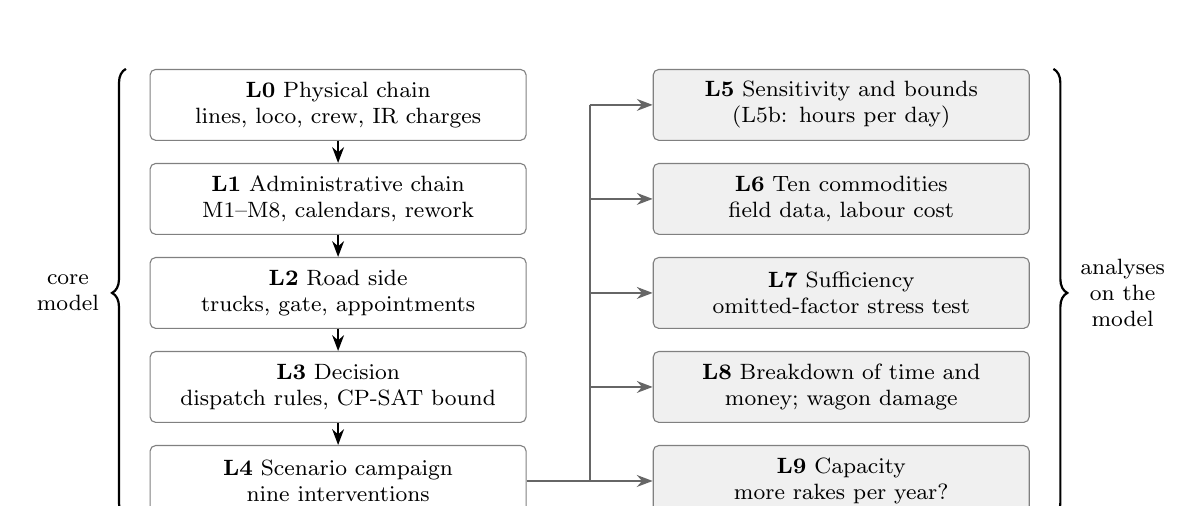
\begin{tikzpicture}[
  font=\footnotesize, >={Stealth[length=2mm]},
  lay/.style={draw=black!50, rounded corners=2pt, minimum height=9mm, text width=46mm, align=center, inner sep=2.5pt},
  ana/.style={draw=black!50, fill=black!6, rounded corners=2pt, minimum height=9mm, text width=46mm, align=center, inner sep=2.5pt},
  node distance=2.8mm and 6mm]
  \node[lay] (l0) {\textbf{L0} Physical chain\\lines, loco, crew, IR charges};
  \node[lay, below=of l0] (l1) {\textbf{L1} Administrative chain\\M1--M8, calendars, rework};
  \node[lay, below=of l1] (l2) {\textbf{L2} Road side\\trucks, gate, appointments};
  \node[lay, below=of l2] (l3) {\textbf{L3} Decision\\dispatch rules, CP-SAT bound};
  \node[lay, below=of l3] (l4) {\textbf{L4} Scenario campaign\\nine interventions};
  \foreach \a/\b in {l0/l1, l1/l2, l2/l3, l3/l4} \draw[->, thick] (\a) -- (\b);
  \node[ana, right=16mm of l0] (l5) {\textbf{L5} Sensitivity and bounds\\(L5b: hours per day)};
  \node[ana, below=of l5] (l6) {\textbf{L6} Ten commodities\\field data, labour cost};
  \node[ana, below=of l6] (l7) {\textbf{L7} Sufficiency\\omitted-factor stress test};
  \node[ana, below=of l7] (l8) {\textbf{L8} Breakdown of time and money; wagon damage};
  \node[ana, below=of l8] (l9) {\textbf{L9} Capacity\\more rakes per year?};
  \draw[decorate, decoration={brace, amplitude=5pt, mirror}, thick] ([xshift=-3mm]l0.north west) -- ([xshift=-3mm]l4.south west)
       node[midway, left=6pt, align=center] {core\\model};
  \draw[decorate, decoration={brace, amplitude=5pt}, thick] ([xshift=3mm]l5.north east) -- ([xshift=3mm]l9.south east)
       node[midway, right=6pt, align=center] {analyses\\on the\\model};
  \coordinate (bus) at ($(l4.east)+(8mm,0)$);
  \draw[thick, black!60] (l4.east) -- (bus);
  \draw[thick, black!60] (bus) -- (bus |- l5.west);
  \foreach \x in {l5, l6, l7, l8, l9} \draw[->, thick, black!60] (bus |- \x.west) -- (\x.west);
\end{tikzpicture}
\caption[Layered construction of the model]{Layered construction of the model. Each core layer (left) is verified before the next is added; the analyses (right, shaded) run on the verified core.}
\label{fig:layers}
\end{figure}

\section{System Description}
\label{sec:system}
Figure~\ref{fig:system} shows the modelled siding. A rake is booked, wagons are allotted, and the empty rake travels to the serving station (\emph{arrival}). It waits for the loading line and the shunting locomotive, is placed on the line (\emph{placement}: the free-time clock starts), is loaded, weighed and reported released (\emph{release}: the clock stops), is removed from the siding (\emph{removal}), and departs once the railway receipt is ready and freight is paid. Only the time from placement to release is billed.

\begin{figure}[!htbp]
\centering
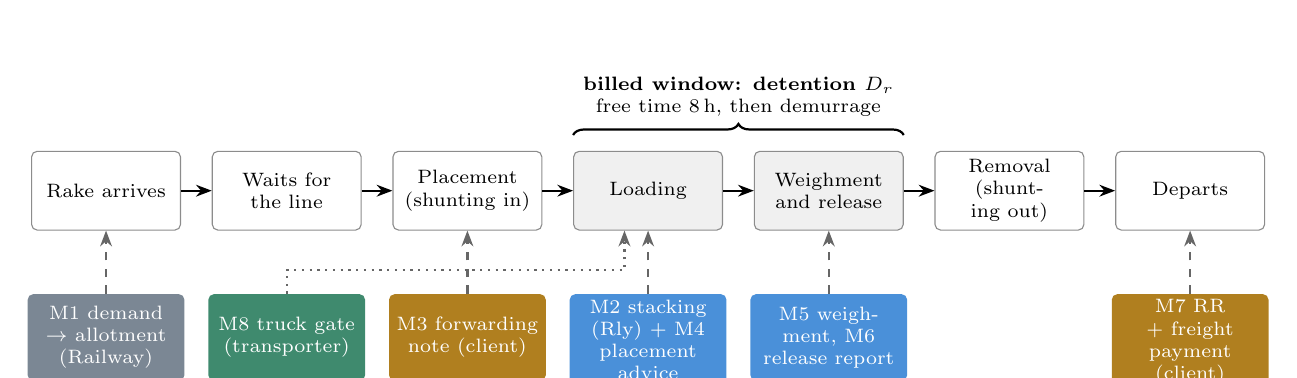
\begin{tikzpicture}[
  font=\scriptsize, >={Stealth[length=2mm]},
  phys/.style={draw=black!45, fill=white, rounded corners=2pt, minimum height=10mm, text width=17.5mm, align=center, inner sep=2pt},
  adm/.style={draw=none, rounded corners=2pt, minimum height=11mm, text width=18.5mm, align=center, inner sep=2pt, text=white},
  node distance=3.9mm]
  \definecolor{term}{HTML}{4A90D9}\definecolor{rail}{HTML}{7B8794}
  \definecolor{clie}{HTML}{B07F1F}\definecolor{tran}{HTML}{3F8A6E}
  \node[phys] (arr) {Rake arrives};
  \node[phys, right=of arr] (wait) {Waits for the line};
  \node[phys, right=of wait] (plc) {Placement (shunting in)};
  \node[phys, right=of plc, fill=black!6] (ld) {Loading};
  \node[phys, right=of ld, fill=black!6] (rel) {Weighment and release};
  \node[phys, right=of rel] (rem) {Removal (shunting out)};
  \node[phys, right=of rem] (dep) {Departs};
  \foreach \a/\b in {arr/wait, wait/plc, plc/ld, ld/rel, rel/rem, rem/dep} \draw[->, thick] (\a) -- (\b);
  \draw[decorate, decoration={brace, amplitude=4pt}, thick] ([yshift=2mm]ld.north west) -- ([yshift=2mm]rel.north east)
     node[midway, above=3pt, align=center] {\textbf{billed window: detention $D_r$}\\free time 8\,h, then demurrage};
  \node[adm, fill=rail, below=8mm of arr] (m1) {M1 demand $\to$ allotment (Railway)};
  \node[adm, fill=tran, below=8mm of wait] (m8) {M8 truck gate (transporter)};
  \node[adm, fill=clie, below=8mm of plc] (m3) {M3 forwarding note (client)};
  \node[adm, fill=term, below=8mm of ld] (m24) {M2 stacking (Rly) + M4 placement advice};
  \node[adm, fill=term, below=8mm of rel] (m56) {M5 weighment, M6 release report};
  \node[adm, fill=clie, below=8mm of dep] (m7) {M7 RR + freight payment (client)};
  \foreach \g/\p in {m1/arr, m3/plc, m24/ld, m56/rel, m7/dep} \draw[->, dashed, thick, black!60] (\g) -- (\p);
  \draw[->, dotted, thick, black!60] (m8.north) -- ++(0,3mm) -| ([xshift=-3mm]ld.south);
\end{tikzpicture}
\caption[The modelled siding]{The modelled siding. Top: physical chain (shaded: IR billed window). Bottom: administrative steps by owner (blue terminal, grey Railway, brown client, green transporter); dashed arrows are gates (the event waits for the document) and the dotted arrow is the road-side supply of material.}
\label{fig:system}
\end{figure}

The twenty-one procedural steps documented in IR rules (five for booking, nine at the siding, four at the truck gate and three at destination) were compressed into the eight administrative steps M1--M8 of Table~\ref{tab:steps}. A step was kept only if it lies on the critical path to placement or release, has a documented approval or rejection loop, and can be traced to an IR rule. Each step has an owner, an office calendar, a lognormal working time and a rejection probability.

\begin{table}[!htbp]
\centering
\caption[The eight administrative steps]{The eight administrative steps. Working times and rejection probabilities are assumed (no published data exist) and tuned to the TERI benchmark; office hours for the terminal shift are cited \cite{ircomp}.}
\label{tab:steps}
\small
\begin{tabularx}{\textwidth}{@{}l X l l c c@{}}
\toprule
\textbf{Step} & \textbf{Task} & \textbf{Owner} & \textbf{Office hours} & \textbf{Mean $\pm$ sd (h)} & \textbf{Rejected} \\
\midrule
M1 & Demand registration to wagon allotment & Railway & 10--17, Mon--Sat & 10.0 $\pm$ 7.0 & 10\,\% \\
M2 & Advance stacking permission & Railway & 10--17, Mon--Sat & 2.0 $\pm$ 1.5 & 15\,\% \\
M3 & Forwarding note acceptance & client & 09--18, Mon--Sat & 1.5 $\pm$ 1.0 & 20\,\% \\
M4 & Placement advice and acknowledgement & terminal & 06--22, daily & 0.5 $\pm$ 0.35 & 5\,\% \\
M5 & Weighment and overload adjustment & terminal & 06--22, daily & 1.8 $\pm$ 1.4 & 18\,\%$^{\dagger}$ \\
M6 & Release reporting & terminal & 06--22, daily & 3.6 $\pm$ 2.8 & 10\,\% \\
M7 & Railway receipt and freight payment & client & 10--17, Mon--Sat & 4.0 $\pm$ 3.0 & 12\,\% \\
M8 & Truck gate verification & transporter & 24/7 & 0.25 $\pm$ 0.12 & 8\,\% \\
\bottomrule
\end{tabularx}
\par\smallskip\raggedright\footnotesize $^{\dagger}$ In the commodity profiles (Layers 6, 8, 9) the M5 rejection rate equals the overload incidence observed in the freight register (30.4\,\% for coal in open wagons).
\end{table}

The physical resources are one loading line, one loading crew and one shunting locomotive, which is needed for placement, removal and detaching wagons. Placement and removal take 1.0 $\pm$ 0.3\,h each (assumed). The road side (Layer 2) brings coal by truck through a gate and a one-way access lane under a truck appointment system; in the base case coal is assumed always available at the siding.

\section{Selection of Variables}
\label{sec:selection}
A candidate factor entered the model only if it passed four filters (Table~\ref{tab:filters}). Twenty-three candidate factors from the literature, the IR rules and the supervisor's guidance were traced through these filters; Table~\ref{tab:factors} summarises where each one sits.

\begin{table}[!htbp]
\centering
\caption[The four filters a factor had to pass to enter the model]{The four filters a factor had to pass to enter the model.}
\label{tab:filters}
\small
\begin{tabularx}{\textwidth}{@{}l X X@{}}
\toprule
\textbf{Filter} & \textbf{Question} & \textbf{Reason} \\
\midrule
F1 Relevance & Does it act on the billed interval (placement to release), or gate its start? & The performance measure is fixed by the Railway's own definition. \\
F2 Evidence & Is it named as a delay cause in TERI, the IR compendium or the dwell-time literature? & No invented mechanisms. \\
F3 Control & Can one of the four parties, or a rule, change it? & The study ranks actions. \\
F4 Measurability & Can it be measured, or bounded by a rule or physical limit? & Every parameter is tagged cited, derived or assumed. \\
\bottomrule
\end{tabularx}
\end{table}

\begin{table}[!htbp]
\centering
\caption[Traceability of the twenty-three candidate factors]{Traceability of the twenty-three candidate factors.}
\label{tab:factors}
\small
\begin{tabularx}{\textwidth}{@{}X p{5.0cm}@{}}
\toprule
\textbf{Candidate factors} & \textbf{Status in the model} \\
\midrule
Rake arrival uncertainty; loading time; line availability; crew availability; locomotive and shunting; office working hours; documents and approvals (M1--M8); weighment and overloading; release reporting; order and payment processing; free time, demurrage and penal rules; road side (trucks, lane, gate); material availability & included (13) \\
Dealing with officials (represented through calendars and rejection rates) & partial (1) \\
Wagon examination and sick-wagon detachment; commodity-specific paperwork; traffic growth; weather and labour absenteeism; higher error rates & left out of the base model, added in the stress test of Layer 7 (5); wagon damage is also an optional module (Layer 8) and traffic growth is studied in Layer 9 \\
Contracts, demurrage pooling and waivers (change the bill, not the time); rake--line length mismatch (acts like a wagon-examination delay); signalling (outside the terminal); wagon life cycle (separate study) & out of scope (4) \\
\bottomrule
\end{tabularx}
\end{table}

The variable set is judged sufficient if the factors it leaves out would not change its conclusions \cite{robinson, sargent}. This is tested directly in Layer 7 (Section~\ref{sec:res_suff}).

\section{Field Data}
\label{sec:data}
The field data are the Eastern Railway inward freight register on the railway-receipt (RR) base: 56 monthly exports from the Freight Operations Information System (FOIS), January 2022 to August 2026 \cite{errr}. After 338 sub-total rows were removed, the register holds 220,395 RRs and 508.5\,Mt. All code columns and charge heads were decoded. The decoding was checked against the charge rules: the terminal charge is exactly Rs 20 per tonne, the busy-season charge is 15\,\%, and coal is exempt from it after 1 October 2022. 220 commodity codes were mapped to 16 groups covering 97\,\% of the tonnes; coal is 61\,\% and iron ore 11\,\%.

The register holds money, tonnes, wagons, wagon type, overloading and charges, but \emph{no placement or release times}. It is therefore used for what it measures: wagons and payload per rake, overload incidence, punitive charges, paid-but-unused capacity, freight per tonne and the arrival pattern. Daily rake arrivals at the 15 largest sidings have a variance-to-mean ratio of 0.7--1.7, close to the value of 1 for a Poisson process, which supports the model's Poisson bookings. Table~\ref{tab:commodities} lists the ten commodity profiles built from the register.

\begin{table}[!htbp]
\centering
\caption[Commodity profiles]{Commodity profiles (Layer 6). Wagons, payload and overload incidence are register medians and shares; free time follows the IR rules; loading rates are assumed by handling method.}
\label{tab:commodities}
\small
\begin{tabular}{@{}lrrlrrr@{}}
\toprule
\textbf{Commodity} & \textbf{Wagons} & \textbf{t/wagon} & \textbf{Loading} & \textbf{t/h} & \textbf{Free time (h)} & \textbf{Overloaded} \\
\midrule
Coal (open BOXN) & 58 & 67.2 & mechanised & 900 & 8 & 30.4\,\% \\
Coal (hopper BOBRN) & 58 & 61.3 & mechanised & 900 & 7 & 40.5\,\% \\
Iron ore & 58 & 68.2 & mechanised & 900 & 7 & 3.7\,\% \\
Clinker & 58 & 68.7 & mechanised & 900 & 7 & 21.4\,\% \\
Cement (bagged) & 42 & 65.7 & manual & 350 & 9 & 1.4\,\% \\
Foodgrains & 42 & 64.9 & manual & 300 & 9 & 0.8\,\% \\
Fertiliser & 42 & 63.8 & manual & 300 & 9 & 1.0\,\% \\
Iron and steel (crane) & 58 & 63.0 & crane & 450 & 9 & 5.3\,\% \\
Containers & 45 & 36.9 & reach-stacker & 600 & 5 & 1.9\,\% \\
POL (tank) & 49 & 54.3 & pumping & 600 & 10 & 0.4\,\% \\
\bottomrule
\end{tabular}
\end{table}

% ----------------------------------------------------------------------
\section{Mathematical Formulation}
\label{sec:form}
The siding is a tandem stochastic system: an administrative stage produces the release dates of a single-machine sequencing problem on the loading line ($1|r_j|\sum C_j$ in the notation of \cite{graham}, with random, calendar-dependent release dates $r_j$). It has no closed-form solution, so the equations below define exactly what the simulation computes, event by event. Table~\ref{tab:notation} lists the main symbols.

\begin{table}[!htbp]
\centering
\caption[Main notation]{Main notation.}
\label{tab:notation}
\small
\begin{tabularx}{\textwidth}{@{}l X l X@{}}
\toprule
\textbf{Symbol} & \textbf{Meaning} & \textbf{Symbol} & \textbf{Meaning} \\
\midrule
$r$ & rake index & $N_w$, $q$, $Q$ & wagons, payload per wagon, tonnes per rake \\
$b_r$, $a_r$ & booking, arrival time & $\lambda$, $R$ & arrival rate (per hour), rakes a year \\
$s_r$, $p_r$ & placement start, placed (clock starts) & $\ell_r$, $e_r$ & loading start, loading end \\
$u_r$ & released (clock stops) & $m_r$, $\delta_r$ & removed (line freed), departed \\
$D_r$, $W_r$ & detention, wait before placement & $H_r$, $\Gamma_r$ & line hold, cycle (arrival to departure) \\
$F$ & free time (8\,h) & $E_r$ & billed excess over free time \\
$T_k(t)$ & completion of step $k$ started at $t$ & $\Phi_k(t,d)$ & calendar operator of step $k$ \\
$\rho_k$ & rejection probability of step $k$ & $K$ & number of loading lines \\
$g_b$, $U_b$ & demurrage rate and upper limit of band $b$ & $\kappa$ & penal multiplier \\
\bottomrule
\end{tabularx}
\end{table}

\subsection{Inputs and Distributions}
Rakes $r = 1,\dots,n$ carry $N_w$ wagons of payload $q$, i.e.\ $Q = N_w q$ tonnes. Bookings form a Poisson stream, $b_r = b_{r-1} + X_r$ with $X_r \sim \mathrm{Exp}(\bar X)$; with $\bar X = 30$\,h the siding receives $R = 8760/\bar X = 292$ rakes a year. Every positive, right-skewed duration (transit $\tau_r$, placement $P_r$, removal $R_r$, loading rate $\mu_r$, paperwork $d_{kr}$) is lognormal and is specified by its real-scale mean $m$ and standard deviation $s$:
\begin{equation}
Y \sim \mathrm{LN}(m,s) \iff \ln Y \sim \mathcal{N}(\mu, \sigma^2), \qquad \sigma^2 = \ln\!\left(1 + s^2/m^2\right), \quad \mu = \ln m - \sigma^2/2 .
\label{eq:logn}
\end{equation}
The loading time is $L_r = Q / \max(\mu_r, \mu_{\min})$, where the floor $\mu_{\min}$ (300\,t/h in the base model) keeps an unlucky draw from producing an impossible loading time. The base model uses the BOXN wagon specification (58 wagons of 58.08\,t); the commodity profiles use the register medians (Table~\ref{tab:commodities}).

\subsection{Office Calendars}
Step $k \in \{\mathrm{M1},\dots,\mathrm{M8}\}$ is worked only while its office is open, $\mathbf{1}_k(t) = 1$. Work of $d$ hours started at time $t$ pauses at closing and resumes at the next opening, so it ends at
\begin{equation}
\Phi_k(t, d) = \min\Big\{ C \ge t : \int_t^{C} \mathbf{1}_k(\tau)\, d\tau = d \Big\}.
\label{eq:cal}
\end{equation}
This operator is the main delay mechanism of the model: a 0.5\,h task started 15 minutes before closing ends the next morning, about 8.5\,h later for the terminal shift. A digitalised or round-the-clock step has $\mathbf{1}_k \equiv 1$, so $\Phi_k(t,d) = t + d$.

\subsection{Rework}
Each submission of step $k$ is rejected with probability $\rho_k$ and redone with a fresh working time. Starting from $C^{(0)} = t$, attempt $j$ ends at $C^{(j)} = \Phi_k\big(C^{(j-1)}, d^{(j)}_{kr}\big)$. The number of attempts $J_{kr}$ is geometric, truncated at five:
\begin{equation}
P(J_{kr} = j) = \rho_k^{\,j-1}(1-\rho_k), \quad j = 1,\dots,4, \qquad P(J_{kr} = 5) = \rho_k^{\,4}, \qquad T_k(t) = C^{(J_{kr})} .
\label{eq:rework}
\end{equation}
Because every attempt passes through the calendar again, a rejection late in the day costs a night, not just the working time of the repeat.

\subsection{Event Recursion (Gates)}
Physical events wait for the documents that gate them. With $\vartheta^{\text{crew}}_r$ and $\vartheta^{\text{loco}}_r$ the times at which the crew and the locomotive become free for rake $r$, the event times are:
\begin{equation}
\begin{aligned}
a_r &= T_{\mathrm{M1}}(b_r) + \tau_r && \text{arrival}\\
s_r &\ge T_{\mathrm{M3}}(a_r) && \text{placement start (dispatch rule, line and loco free)}\\
p_r &= s_r + P_r && \text{placed: IR free-time clock starts}\\
\ell_r &= \max\{T_{\mathrm{M4}}(p_r),\; T_{\mathrm{M2}}(b_r),\; \vartheta^{\text{crew}}_r\} && \text{loading start}\\
e_r &= \ell_r + L_r && \text{loading end}\\
u_r &= T_{\mathrm{M6}}\big(T_{\mathrm{M5}}(e_r)\big) && \text{released: clock stops}\\
m_r &= \max\{u_r, \vartheta^{\text{loco}}_r\} + R_r && \text{removed: line freed}\\
\delta_r &= \max\{m_r,\; T_{\mathrm{M7}}(e_r)\} && \text{departure (RR and payment done)}
\end{aligned}
\label{eq:chain}
\end{equation}
M2 starts at booking and M7 at loading end, in parallel with the physical chain. The capacity constraint is that at most $K$ of the intervals $[s_r, m_r)$ overlap at any time ($K = 1$ line in the base case).

\subsection{Performance Measures and IR Charges}
For each rake, detention, waiting, line hold and cycle time are
\begin{equation}
D_r = u_r - p_r, \qquad W_r = s_r - a_r, \qquad H_r = m_r - s_r, \qquad \Gamma_r = \delta_r - a_r .
\label{eq:kpi}
\end{equation}
The billed excess is $E_r = \lceil D_r - F \rceil^{+}$ with free time $F = 5 + 2 + 1 = 8$\,h, and demurrage per rake is the graded charge \cite{ircomp}
\begin{equation}
\mathrm{Dem}_r = \kappa\, N_w \sum_{b=1}^{6} g_b \big[\min(E_r, U_b) - U_{b-1}\big]^{+},
\label{eq:dem}
\end{equation}
with band limits $U = (0, 6, 12, 24, 48, 72, \infty)$\,h, rates $g_b = 150 \times (1, 1.1, 1.25, 1.5, 2, 3)$ Rs per wagon-hour (Table~\ref{tab:bands}) and penal multiplier $\kappa$ (1 in the base case, up to 6). Because $g_b$ rises with $b$, Eq.~\eqref{eq:dem} is piecewise linear and convex in $E_r$: the last hour of detention is the dearest, so a cut in hours removes demurrage more than proportionally. The share of rakes over free time is the mean of $\mathbf{1}[E_r > 0]$.

Three further measures convert hours into wagons and money:
\begin{equation}
\Delta W = \frac{R\, N_w\, \Delta\bar\Gamma}{8760}, \qquad
\Theta = \theta_{\text{ov}}\, C_{\text{pun}} + Q_{\text{u}}\, f, \qquad
B = -\frac{\Delta\overline{\mathrm{Dem}}}{Q} .
\label{eq:derived}
\end{equation}
$\Delta W$ is the number of wagons returned to the fleet when the mean cycle falls by $\Delta\bar\Gamma$ (Little's law \cite{little}: wagons tied up = arrival rate $\times$ time in system), valued at Rs 1,140 crore / 2,583 per wagon from a recent wagon order \cite{wagonvalue}. $\Theta$ is the loss per rake measured in the register: overload incidence $\theta_{\text{ov}}$ times the punitive charge $C_{\text{pun}}$, plus paid-but-unused tonnes $Q_{\text{u}}$ times freight $f$ per tonne. $B$ is the labour break-even per tonne: the most that can be spent per tonne on 50\,\% faster loading before it costs more than the demurrage it avoids. Each segment of $\Gamma_r$ is owned by one party (Figure~\ref{fig:system}), and a party's share is the sum of its segments over the total.

\subsection{Capacity of the Siding}
With $K$ lines, each held $\bar H$ hours per rake, the most rakes the siding can turn round in a year is the \emph{capacity ceiling}
\begin{equation}
\Lambda_K = \frac{K \cdot 8760}{\bar H} .
\label{eq:ceiling}
\end{equation}
At the ceiling the lines are busy 100\,\% of the time and the queue grows without limit, so the ceiling is never a workable traffic level. The workable level is measured by raising the offered traffic $R$ and recording the mean wait $\bar W(R)$. The \emph{same-service capacity} of a configuration is the largest traffic it can accept while keeping the wait no longer than the siding's wait today:
\begin{equation}
R^{*} = \max\big\{ R : \bar W(R) \le \bar W_{\text{today}}(292) \big\},
\label{eq:samesvc}
\end{equation}
found by linear interpolation between simulated traffic levels. No new threshold is assumed: today's service is the yardstick. The utilisation of each resource at traffic $R$ shows what saturates first: line $\rho_{\text{line}} = R \bar H / (K \cdot 8760)$, crew $R \bar L / (c \cdot 8760)$ for $c$ crews, and locomotive $R(\bar P + \bar R)/8760$.

The single-line queue is checked against queueing theory. For Poisson arrivals at rate $\lambda$ and line holds $S$ with $\rho = \lambda E[S] < 1$, the Pollaczek--Khinchine formula gives the mean wait in queue \cite{gross}
\begin{equation}
W_q = \frac{\lambda\, E[S^2]}{2(1 - \rho)} .
\label{eq:pk}
\end{equation}

\subsection{Dispatch and Optimisation}
When a line frees at time $t$, the waiting rake with the lowest priority index is placed, $r^* = \arg\min_{r \in \mathcal{W}(t)} \pi(r, t)$, ties broken by rake number. First-come-first-served (FCFS) uses $\pi = a_r$ and shortest processing time (SPT) uses $\pi = L_r$. The Contract Net bid \cite{smith} is the rake's expected demurrage plus its line-blocking cost ($c_I$, an assumed idle cost of Rs 3,000 per hour) minus an ageing credit that prevents starvation; the cost rule is the same bid without ageing ($\alpha = 0$):
\begin{equation}
\pi_{\text{CNP}}(r,t) = g_1 N_w (P_r + L_r - F)^{+} + c_I (P_r + L_r + R_r) - \alpha\, c_I\, (t - a_r), \qquad \alpha = 0.5 .
\label{eq:cnp}
\end{equation}
The offline benchmark, solved with the CP-SAT solver \cite{ortools} in integer minutes, knows every arrival and line hold $h_r$ in advance:
\begin{equation}
\min \sum_{r} (S_r - a_r) \quad \text{s.t.} \quad S_r \ge a_r \;\; \forall r, \qquad \textsc{NoOverlap}\big\{[S_r,\, S_r + h_r)\big\}_r ,
\label{eq:cpsat}
\end{equation}
with \textsc{Cumulative} $\le K$ in place of \textsc{NoOverlap} for $K > 1$ lines. For a valid lower bound $LB$ on the mean wait of any policy, $h_r$ is replaced by $\underline{h}_r$, the hold of rake $r$ with every calendar open and no rework (a closure or a rejection never shortens a step), and the solver's proven bound divided by $n$ is reported. Waiting is then split with counterfactual runs without calendars, without rework, and without both (``flat''):
\begin{equation}
\underbrace{1 - \tfrac{\bar W_{\text{flat}}}{\bar W}}_{\text{administrative}} \;+\; \underbrace{\tfrac{\bar W_{\text{flat}} - LB}{\bar W}}_{\le\ \text{sequencing}} \;+\; \underbrace{\tfrac{LB}{\bar W}}_{\text{irreducible}} = 1,
\label{eq:wsplit}
\end{equation}
with office hours alone $1 - \bar W_{\text{nocal}}/\bar W$ and rework alone $1 - \bar W_{\text{norw}}/\bar W$.

\subsection{Statistical Design and Analysis}
Each random stream is seeded by a BLAKE2b hash of the replication seed and a name keyed on the rake and the step (for example, the M5 working time of rake 17). Every scenario therefore sees the same rakes with the same draws (common random numbers), and a change in one scenario cannot reshuffle the draws of other rakes. A scenario is compared with its base by the paired difference over $n_R$ replications,
\begin{equation}
\bar\Delta \pm 1.96\, \frac{s_\Delta}{\sqrt{n_R}},
\label{eq:ci}
\end{equation}
and is called significant when the interval excludes zero \cite{law}. For bounds, factor $i$ is set alone to each level $x_i^{(l)}$ of its range (the rule's own range for cited parameters, published limits for the loading rate, $\pm 50$\,\% for assumed ones) and its swing is $\max_l \bar y(x_i^{(l)}) - \min_l \bar y(x_i^{(l)})$; a best/worst envelope sets all factors at their favourable or unfavourable ends at once. Morris screening \cite{morris, campolongo} uses the unit cube with four levels, step $\Delta = 2/3$ and $R_M = 20$ trajectories:
\begin{equation}
EE_i = \frac{y(\mathbf{x} + \Delta \mathbf{e}_i) - y(\mathbf{x})}{\Delta}, \qquad \mu_i^{*} = \frac{1}{R_M}\sum |EE_i|, \qquad \sigma_i = \mathrm{sd}(EE_i),
\label{eq:morris}
\end{equation}
where $\mu^*$ measures importance and $\sigma$ interaction or non-linearity. Detention is split by cause through counterfactual runs; the terms telescope, so the split is exact:
\begin{equation}
\bar D = \underbrace{\bar L}_{\text{loading}} + \underbrace{(\bar D_{\text{flat}} - \bar L)}_{\text{paperwork time}} + \underbrace{(\bar D_{\text{nocal}} - \bar D_{\text{flat}})}_{\text{rework}} + \underbrace{(\bar D - \bar D_{\text{nocal}})}_{\text{waiting for office}} .
\label{eq:dsplit}
\end{equation}
Levers in a package overlap, so lever $i$ of a package $N$ with $n$ levers receives its Shapley value \cite{shapley}, its average marginal saving over all orders of introduction, computed from a full factorial of simulated lever sets. The shares add up exactly to the package's saving, $\sum_i \phi_i = v(N)$:
\begin{equation}
\phi_i = \sum_{S \subseteq N \setminus \{i\}} \frac{|S|!\,(n - |S| - 1)!}{n!} \big[v(S \cup \{i\}) - v(S)\big], \qquad v(S) = \bar D_{\text{today}} - \bar D(S),
\label{eq:shapley}
\end{equation}
Sufficiency is judged by Kendall's rank correlation $\tau_a = (n_c - n_d)/\binom{m}{2}$ between the ranking of the $m$ interventions in a stress scenario and in the model as built \cite{kendall}, where $n_c$ and $n_d$ are the concordant and discordant pairs.

\subsection{Wagon Damage (Optional Module)}
At placement $N^{\text{def}}_r \sim \mathrm{Bin}(N_w, p)$ wagons are found defective; each is minor, repairable or unfit with probabilities 0.6, 0.3 and 0.1. Repairs (each $\mathrm{LN}(1.5, 0.75)$\,h) and the detaching of $k_r = \min(N^{\text{unfit}}_r, N_w - 1)$ unfit wagons ($\mathrm{LN}(1.5, 0.5)$\,h, needs the locomotive) run beside M4, so loading starts at the latest of $T_{\mathrm{M4}}(p_r)$, $T_{\mathrm{M2}}(b_r)$ and $p_r + \sum_i H_{ir} + G_r$, and lasts $L_r (N_w - k_r)/N_w$. Under the \emph{return} policy a rake with unfit wagons is sent back before its clock starts and replaced after an $\mathrm{LN}(24, 12)$\,h lead time (at most three attempts). Damage during loading, $\mathrm{Bin}(N_w, p')$, is repaired ($\mathrm{LN}(1.0, 0.5)$\,h each) beside M5--M6, so $u_r = \max\{T_{\mathrm{M6}}(T_{\mathrm{M5}}(e_r)),\; e_r + \sum_i H'_{ir}\}$. All damage rates and times are assumed; the module is off by default and changes nothing when off.

% ----------------------------------------------------------------------
\section{Parameters and Calibration}
\label{sec:params}
Every parameter carries a provenance tag: 18 are \emph{cited}, 1 is \emph{derived} and 10 are \emph{assumed} (Table~\ref{tab:prov}). Results that depend only on cited and derived values are quoted as figures; results that touch an assumed value are reported as directions and rankings.

\begin{table}[!htbp]
\centering
\caption[Provenance of the main parameters]{Provenance of the main parameters.}
\label{tab:prov}
\small
\begin{tabularx}{\textwidth}{@{}p{4.4cm} X p{4.2cm}@{}}
\toprule
\textbf{Parameter} & \textbf{Value} & \textbf{Status / source} \\
\midrule
Free time, coal, private siding & 5\,h + 2\,h siding + 1\,h tarpaulin = 8\,h & derived from \cite{ircomp} \\
Graded demurrage; penal & Rs 150--450 per wagon-h by band; up to $6\times$ & cited \cite{ircomp} \\
Terminal working hours & 06:00--22:00 & cited \cite{ircomp} \\
Rake (BOXN), base model & 58 wagons $\times$ 58.08\,t & cited (wagon specification) \\
Detention benchmark & 14--17\,h per rake (calibration target) & cited \cite{teri} \\
Commodity profiles & wagons, payload, overloading, freight & field data \cite{errr} \\
Loading rate & 900\,t/h (range 675--3,370\,t/h) & assumed; range published \cite{pib} \\
Placement, removal & 1.0 $\pm$ 0.3\,h each & assumed \\
M1--M8 working times; rework & Table~\ref{tab:steps} & assumed (no published data) \\
Idle cost, engine-hour cost, shunting charge & Rs 3,000/h; Rs 6,000/h; Rs 25,000 & assumed (cost rule only; not in demurrage) \\
\bottomrule
\end{tabularx}
\end{table}

The assumed working times of M1--M8 were tuned so that the calibrated base lands inside TERI's 14--17\,h band. This is \emph{calibration}, not validation: the band was a target, so agreement with it is weak evidence. The model was, however, checked against facts it was not tuned to: Poisson arrivals and the charge rules in the field data (Section~\ref{sec:data}), and queueing theory (Section~\ref{sec:res_capacity}).

% ----------------------------------------------------------------------
\section{Experimental Design}
\label{sec:design}
Unless stated otherwise, each scenario runs 50 rakes (the first 5 discarded as warm-up) in each of 30 replications, with common random numbers and FCFS dispatch. Layers 3 and 4 use a more congested operating point, so that sequencing has something to act on: 25 rakes per replication arriving every 22\,h on average (line utilisation about 0.7), with 10 replications (12 for the waiting split). The capacity study uses 200 rakes per replication (first 20 discarded), so that long queues can build up. Table~\ref{tab:experiments} lists the experiments.

\begin{table}[!htbp]
\centering
\caption[Experiments by layer]{Experiments by layer. Every output file is regenerated by code (\texttt{run\_all.sh}).}
\label{tab:experiments}
\small
\begin{tabularx}{\textwidth}{@{}l X X@{}}
\toprule
\textbf{Layer} & \textbf{Question} & \textbf{Design} \\
\midrule
L0--L1 & What does the base siding do, and who owns each hour? & calibrated base; attribution by owner \\
L3 & Can better sequencing help? & FCFS, SPT, cost rule, Contract Net, CP-SAT lower bound; waiting split, Eq.~\eqref{eq:wsplit} \\
L4 & Which interventions save most? & nine interventions, paired against the base \\
L5, L5b & What is the individual effect of every factor? & 39 parameters and 27 conditions alone; Morris; envelope; every terminal day length from 8 to 24\,h \\
L6 & Do the levers hold for other commodities, and does labour pay? & ten commodity profiles; labour break-even, Eq.~\eqref{eq:derived} \\
L7 & Is the variable set sufficient? & eight omitted-factor scenarios; Kendall $\tau$ \\
L8 & Where do the hours and the rupees come from? & packages Today, A, B, C; cause split; IR bands; $2^5$ factorial; Shapley; parties; wagon damage \\
L9 & How many more rakes can the siding take? & six configurations $\times$ traffic from 250 to 1,600 rakes a year; ceiling, same-service capacity, utilisations; Pollaczek--Khinchine check \\
\bottomrule
\end{tabularx}
\end{table}

The packages of Layers 8 and 9 combine four levers: \textbf{H}, terminal paperwork (M4--M6) round the clock; \textbf{D}, digital release reporting (M6 with no office hours, no rejections and half the working time); \textbf{P}, precise loading (no overloading, hence no weighment rework); and \textbf{L}, loading 50\,\% faster. Package \textbf{A} = H + D needs no construction; \textbf{B} = A + P; \textbf{C} = B + L.

% ----------------------------------------------------------------------
\section{Implementation and Verification}
\label{sec:impl}
The model is implemented as the Python package \texttt{rtsim} (SimPy for the event engine, pandas and NumPy for analysis, OR-Tools CP-SAT for the bound, Matplotlib for charts) with one runner script per layer. The code, the decoded data and every result table are kept in a version-controlled repository; a single script, \texttt{run\_all.sh}, regenerates every result from scratch, and results are never edited by hand.

\begin{table}[!htbp]
\centering
\caption[Main code modules]{Main code modules.}
\label{tab:code}
\small
\begin{tabularx}{\textwidth}{@{}l X@{}}
\toprule
\textbf{Module} & \textbf{Role} \\
\midrule
\texttt{config.py}, \texttt{calibration.py} & all parameters with their provenance tags \\
\texttt{distributions.py}, \texttt{experiment.py} & lognormal and other draws; entity-keyed random streams; replications \\
\texttt{terminal.py}, \texttt{admin.py} & physical chain, gates, M1--M8, calendars and rework, Eqs.~\eqref{eq:cal}--\eqref{eq:chain} \\
\texttt{accounting.py} & detention, demurrage by band and attribution, Eqs.~\eqref{eq:kpi}--\eqref{eq:dem} \\
\texttt{policies.py}, \texttt{optimiser.py} & dispatch rules, Contract Net and CP-SAT, Eqs.~\eqref{eq:cnp}--\eqref{eq:cpsat} \\
\texttt{trucks.py}, \texttt{damage.py} & road side and the optional wagon-damage module \\
\texttt{experiments/run\_layer*.py} & one runner per layer (Table~\ref{tab:experiments}) \\
\texttt{tools/rr\_register.py} & decoding of the freight register \\
\bottomrule
\end{tabularx}
\end{table}

Verification follows the standard practice of checking that the model does what it is meant to do \cite{sargent}. One hundred and seven automated checks run after every change, and all pass. They include:
\begin{itemize}
    \item \textbf{Invariants:} every rake that arrives also leaves; events of every rake occur in order; the line is never over capacity; physical durations do not depend on the dispatch rule; every event carries a party owner; Little's law holds within 5\,\%; no dispatch rule beats the CP-SAT lower bound.
    \item \textbf{Layer consistency:} switching a layer off reproduces the layer below exactly; the damage module with zero damage reproduces the model exactly.
    \item \textbf{Exact sums:} the cause split adds up to detention; demurrage by band adds up to demurrage per rake; Shapley shares add up to each package's saving.
    \item \textbf{Directions:} longer terminal hours never increase detention; more damage never shortens it; the queue never shrinks when more rakes are offered; a second line roughly doubles the capacity ceiling.
    \item \textbf{Field data:} no sub-total rows remain; tonnage is conserved; the decoded charges equal the rules.
    \item \textbf{Theory:} with all offices open, the simulated queue matches the Pollaczek--Khinchine formula, Eq.~\eqref{eq:pk}.
\end{itemize}
A refactor is accepted only if it reproduces every earlier result table exactly.

% ======================================================================
% CHAPTER 3  RESULTS AND DISCUSSION
% ======================================================================
\chapter{Results and Discussion}
\label{ch:results}
This chapter follows the questions of Table~\ref{tab:experiments}. All figures and tables are regenerated by code from the committed result files, and every comparison is paired under common random numbers. Results that rest on assumed parameters are read as directions and rankings (Section~\ref{sec:params}).

\section{Calibrated Baseline}
\label{sec:res_base}
The calibrated base (coal, BOXN wagons, 292 rakes a year) gives a mean detention of \textbf{15.53 $\pm$ 0.33\,h} per rake, inside TERI's 14--17\,h band, while the physical chain alone (Layer 0, no paperwork) gives 4.05\,h. Of the rakes, 84\,\% exceed the 8\,h free time. Table~\ref{tab:attrib} shows who owns each hour of a rake's time at the siding: the terminal owns 73.5\,\%, the client 23.7\,\% and the Railway 2.9\,\%. Half of all rake time is spent queueing for the line, and the railway receipt and payment (client) take almost a quarter.

\begin{table}[!htbp]
\centering
\caption[Attribution of rake time by segment and owner, calibrated base]{Attribution of rake time by segment and owner, calibrated base (Layer 1, 50 rakes).}
\label{tab:attrib}
\small
\begin{tabular}{@{}llrr@{}}
\toprule
\textbf{Segment} & \textbf{Owner} & \textbf{Mean per rake (h)} & \textbf{Share} \\
\midrule
Queueing for the line & terminal & 35.45 & 51.0\,\% \\
Railway receipt and payment (M7) & client & 16.45 & 23.7\,\% \\
Release reporting (M5, M6) & terminal & 9.78 & 14.1\,\% \\
Loading & terminal & 4.14 & 6.0\,\% \\
Waiting for the crew & terminal & 1.69 & 2.4\,\% \\
Placement shunting & Railway & 1.01 & 1.5\,\% \\
Removal shunting & Railway & 0.97 & 1.4\,\% \\
\midrule
\multicolumn{2}{@{}l}{\textbf{Total by owner:} terminal 73.5\,\%, client 23.7\,\%, Railway 2.9\,\%} & & 100\,\% \\
\bottomrule
\end{tabular}
\end{table}

The client's share depends on the assumption that the railway receipt (M7) waits for railway office hours. The field data show electronic receipts for 99.7\,\% of coal, so in practice the client's share is smaller; this affects wagon time and attribution but not detention or demurrage, because M7 lies outside the billed window (Section~\ref{sec:res_break}).

\section{Where Detention Comes From}
\label{sec:res_where}
In a congested test case (one rake every 22\,h), the waiting split of Eq.~\eqref{eq:wsplit} gives:
\begin{itemize}
    \item \textbf{about 78\,\% administrative}: removing office hours alone removes 73.3\,\% of rake waiting, removing rework alone 10.9\,\%, and removing both 77.8\,\%;
    \item \textbf{at most 8\,\%} recoverable by optimal sequencing (the CP-SAT lower bound);
    \item \textbf{14\,\%} irreducible congestion, which no sequence can avoid.
\end{itemize}
Accordingly, no online dispatch rule beats first-come-first-served significantly at this operating point: SPT, the cost rule and Contract Net all give the same mean wait within their confidence intervals. Dispatch matters for \emph{fairness}, not for the mean: the cost rule without ageing lets the worst rake wait 161.2\,h, and Contract Net with ageing ($\alpha = 0.5$) cuts that to 108.1\,h ($-33$\,\%) at an unchanged mean wait. The lesson is that rakes wait mainly for offices and documents, not because they are served in the wrong order.

\section{Procedural versus Capital Interventions}
\label{sec:res_interv}
Figure~\ref{fig:interv} ranks the interventions against the campaign's own paired base (16.07\,h at the congested operating point of Section~\ref{sec:design}); opening every office round the clock gives the same detention as the terminal working round the clock and is not drawn separately. The three paperwork levers each save more than any capital lever. Digitalising the paperwork saves 8.98\,h per rake and cuts the share of rakes over free time from 86.8\,\% to 24.5\,\%; a second line with a second crew saves 0.58\,h, a factor of about 15.5. A second loading line \emph{alone} does not help (+0.28\,h, not significant), because with one crew two rakes compete for it, and a second shunting locomotive changes nothing, because shunting lies outside the billed window.

\begin{figure}[!htbp]
\centering
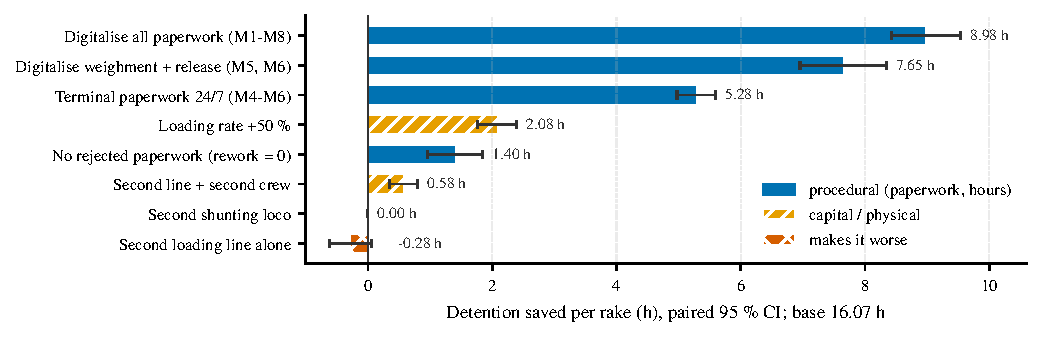
\includegraphics[width=0.94\textwidth]{figures/fig_interventions.pdf}
\caption[Detention saved per rake by each intervention]{Detention saved per rake by each intervention (Layer 4, 10 paired replications $\times$ 25 rakes, one rake every 22\,h). Procedural levers dominate; a second line without a crew does not help.}
\label{fig:interv}
\end{figure}

Detention, however, is only the billed window. A second line with a second crew barely shortens detention, but it cuts the \emph{wait before placement} from 44.3 to 17.2\,h, because two rakes can now be served at once. Procedural and capital levers therefore act on different things: procedure shortens each rake's stay on the line, while a second line adds a second place to stand. This difference becomes decisive for capacity (Section~\ref{sec:res_capacity}).

\section{Individual Effect of Every Factor}
\label{sec:res_sens}
Thirty-nine parameters and 27 conditions were varied one at a time over stated ranges (Figure~\ref{fig:sens}a). One calendar decision dominates: the number of hours a day the terminal's own paperwork (M4--M6) runs moves detention from 31.86\,h (8\,h a day) to 10.69\,h (24\,h a day), a swing of 21.2\,h, more than all physical parameters together. Release reporting (M6) and the loading rate follow, at 6.6\,h each. Each extra terminal hour helps less than the one before (Figure~\ref{fig:sens}b); extending today's 16\,h to 18\,h already yields 43\,\% of the round-the-clock gain (2.07 of 4.84\,h).

\begin{figure}[!htbp]
\centering
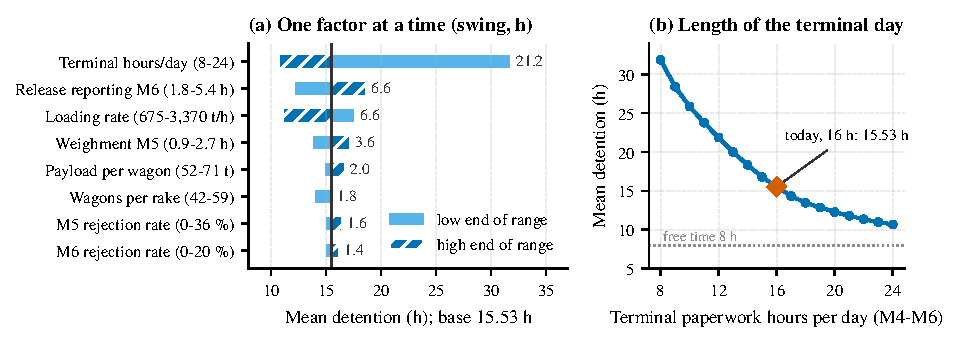
\includegraphics[width=0.94\textwidth]{figures/fig_sensitivity.pdf}
\caption[Individual effect of the top factors and of the length of the terminal day]{(a) Mean detention at the low and high end of each factor's range, top eight factors (number = swing in hours). (b) Detention for every length of the terminal paperwork day, with 95\,\% band (Layers 5 and 5b).}
\label{fig:sens}
\end{figure}

Morris screening (Figure~\ref{fig:morris}) confirms the same top three factors, terminal hours, M6 release time and the loading rate, followed by M5 weighment time. Their large $\sigma$ shows that their effects interact with other factors, which is why lever savings overlap (Section~\ref{sec:res_break}). All remaining parameters have $\mu^* < 2$\,h. Among the conditions, removing the release-reporting step entirely would save 6.55\,h, and two lines with two crews save only 0.67\,h of detention but 17.7\,h of waiting. Commercial parameters move money only: the penal multiplier raises demurrage per rake from Rs 75,962 to Rs 4.56 lakh at unchanged detention, so pricing cannot release a rake faster. With every factor at its favourable or unfavourable end, detention spans 3.54 to 51.41\,h.

\begin{figure}[!htbp]
\centering
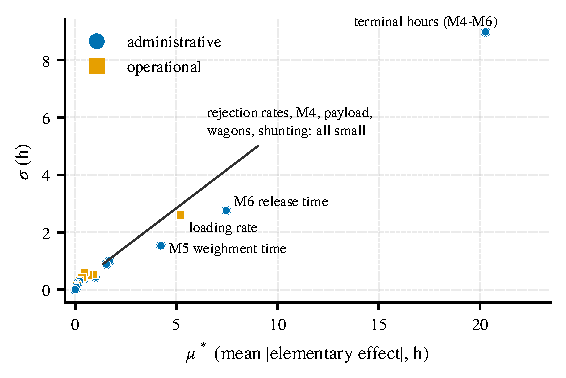
\includegraphics[width=0.62\textwidth]{figures/fig_morris.pdf}
\caption[Morris screening of the 39 parameters]{Morris screening of the 39 parameters ($R_M = 20$ trajectories, Eq.~\eqref{eq:morris}). Importance $\mu^*$ against interaction $\sigma$.}
\label{fig:morris}
\end{figure}

\section{Materials and Labour}
\label{sec:res_comm}
The ten commodity profiles of Table~\ref{tab:commodities} give base detentions from 13.4\,h (containers) to 22.0\,h (foodgrains); manual loading of bagged cargo makes loading itself long. Figure~\ref{fig:commodity} and Table~\ref{tab:levers} show how each lever acts on each material. Round-the-clock terminal paperwork and digital release help every material by a similar amount. Faster loading and digital weighment help all materials, by an amount that depends on the material. Silo loading and precise loading matter mainly for bulk, where overloading is frequent, and a second line with a crew changes sign across materials.

\begin{figure}[!htbp]
\centering
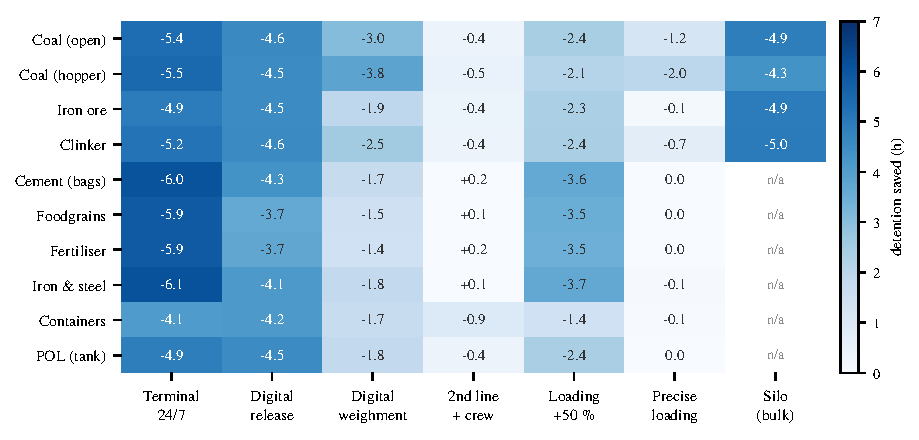
\includegraphics[width=0.94\textwidth]{figures/fig_commodity.pdf}
\caption[Change in detention per rake (h) for each lever and commodity]{Change in detention per rake (h) for each lever and commodity (Layer 6, paired against each commodity's own base). Silo loading applies only to mechanised bulk.}
\label{fig:commodity}
\end{figure}

\begin{table}[!htbp]
\centering
\caption[Change in detention per rake (h) across the ten commodity profiles, with the class of each lever]{Change in detention per rake (h) across the ten commodity profiles, with the class of each lever.}
\label{tab:levers}
\small
\begin{tabular}{@{}lcl@{}}
\toprule
\textbf{Lever} & \textbf{Range (h)} & \textbf{Class} \\
\midrule
Terminal paperwork 24/7 (M4--M6) & $-4.1$ to $-6.1$ & general, uniform \\
Digital release reporting (M6) & $-3.7$ to $-4.6$ & general, uniform \\
Loading rate $+50$\,\% & $-1.4$ to $-3.7$ & general, size depends on material \\
Digital weighment (M5) & $-1.4$ to $-3.8$ & general, size depends on material \\
Silo / rapid loading (bulk only) & $-4.3$ to $-5.0$ & material-specific \\
Precise loading (no overload) & $0.0$ to $-2.0$ & material-specific \\
Second line + second crew & $+0.2$ to $-0.9$ & material-specific (sign changes) \\
\bottomrule
\end{tabular}
\end{table}

\paragraph{Labour versus demurrage.} Loading 50\,\% faster can be bought with more labour. The labour break-even $B$ of Eq.~\eqref{eq:derived} is the most that can be spent per tonne before the extra labour costs more than the demurrage it avoids. It is about Rs 5.5 per tonne for mechanised bulk and Rs 9 per tonne for bagged cargo, i.e.\ about 46\,\% of the published coal handling rate and about 10\,\% of the bagged-cargo handling rate \cite{cwc}. Extra labour therefore pays for every material when it is paid per tonne. Paid per shift, it roughly breaks even for bulk and loses money for bagged cargo, because manual handling is already expensive per tonne.

\section{Breakdown of Time and Money}
\label{sec:res_break}
For the dominant real case, coal in open wagons at 292 rakes a year (register profile), four packages were simulated (Section~\ref{sec:design}): \emph{Today}; \emph{A}, terminal paperwork 24/7 plus digital release reporting, which needs no construction; \emph{B}, A plus precise loading; and \emph{C}, B plus 50\,\% faster loading.

\subsection{Where the Hours Come From}
Figure~\ref{fig:break}a splits the billed window exactly by cause (Eq.~\eqref{eq:dsplit}). Today, 6.5 of the 17.0\,h (38\,\%) are not productive work: 5.4\,h of waiting for an office to open and 1.1\,h of redoing rejected documents. Package A removes the office wait almost entirely; precise loading removes the remaining rework; faster loading then shortens the physical part. The bottleneck therefore \emph{moves}, from office hours to paperwork working time to loading speed, and each package attacks the next one.

\begin{figure}[!htbp]
\centering
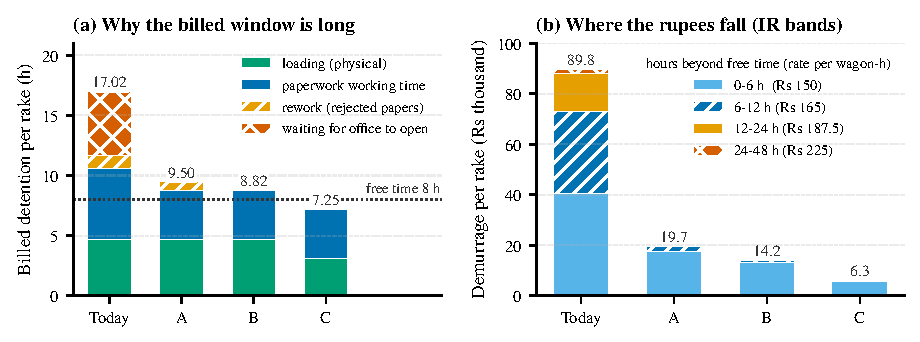
\includegraphics[width=0.94\textwidth]{figures/fig_breakdown.pdf}
\caption[Breakdown of billed detention and demurrage per package, coal siding]{Coal rake in open BOXN wagons, packages Today, A, B, C (Layer 8). (a) Billed detention split exactly by cause. (b) Demurrage per rake by IR charge band.}
\label{fig:break}
\end{figure}

\subsection{Where the Rupees Come From}
Money falls faster than time (Figure~\ref{fig:break}b and Table~\ref{tab:pack}), as the convexity of Eq.~\eqref{eq:dem} predicts. Package A cuts detention by 44\,\% but demurrage by 78\,\%, because every hour removed lies above the free time and the dearer bands empty first: under A the 6--12\,h band falls from Rs 32,262 to Rs 1,900 per rake and the 12--24\,h band from Rs 15,152.5 to Rs 209. Over a year of 292 rakes, package A avoids Rs 2.05 crore of demurrage, B Rs 2.21 crore and C Rs 2.44 crore.

\begin{table}[!htbp]
\centering
\caption[Outcomes per package, coal siding, 292 rakes a year]{Outcomes per package, coal siding, 292 rakes a year (Layer 8, means of 30 replications $\times$ 50 rakes). Wagons freed assume electronic railway receipts, as the field data show for coal.}
\label{tab:pack}
\small
\begin{tabular}{@{}lrrrr@{}}
\toprule
 & \textbf{Today} & \textbf{A} & \textbf{B} & \textbf{C} \\
\midrule
Detention per rake (h) $\downarrow$ & 17.02 & 9.50 & 8.82 & 7.25 \\
Rakes over free time (\%) $\downarrow$ & 90 & 67 & 59 & 28 \\
Wait before placement (h) $\downarrow$ & 37.4 & 20.2 & 19.4 & 17.9 \\
Line held per rake (h) $\downarrow$ & 19.0 & 11.5 & 10.8 & 9.2 \\
Demurrage per rake (Rs) $\downarrow$ & 89,786 & 19,651 & 14,195 & 6,265 \\
Demurrage avoided (Rs crore/yr) $\uparrow$ & -- & 2.05 & 2.21 & 2.44 \\
Overload and unused capacity (Rs crore/yr) $\uparrow$ & -- & -- & 4.20 & 4.20 \\
Wagons freed (Rs crore) $\uparrow$ & -- & 47.6 (21.0) & 50.5 (22.3) & 56.4 (24.9) \\
\bottomrule
\end{tabular}
\end{table}

Precise loading also removes the register-measured loss $\Theta$ (Eq.~\eqref{eq:derived}) of Rs 1.44 lakh per rake, Rs 4.20 crore a year. Most of it is paid-but-unused wagon capacity, i.e.\ about 159\,t more coal per rake for the same freight, so it is a capacity gain rather than cash.

\subsection{Fair Split between Levers}
The levers overlap: alone they would save 13.51\,h, together they save 9.77\,h. Table~\ref{tab:shapley} gives the Shapley split (Eq.~\eqref{eq:shapley}) of package C. Terminal hours and digital release together account for 71\,\% of the saving, and both need no construction.

\begin{table}[!htbp]
\centering
\caption[Saving of package C per rake: each lever alone and its Shapley share]{Saving of package C per rake: each lever alone and its Shapley share (Layer 8, $2^5$ factorial).}
\label{tab:shapley}
\small
\begin{tabular}{@{}lrrrr@{}}
\toprule
\textbf{Lever} & \textbf{Alone (h)} & \textbf{Shapley (h)} & \textbf{Share} & \textbf{Shapley (Rs per rake)} \\
\midrule
H Terminal paperwork 24/7 & 5.35 & 3.66 & 37\,\% & 33,613 \\
D Digital release reporting & 4.59 & 3.30 & 34\,\% & 28,265 \\
L Loading 50\,\% faster & 2.39 & 1.89 & 19\,\% & 13,955 \\
P Precise loading & 1.18 & 0.91 & 9\,\% & 7,689 \\
\midrule
\textbf{Total} & 13.51 & 9.77 & 100\,\% & 83,521 \\
\bottomrule
\end{tabular}
\end{table}

\subsection{Who Gains What}
The demurrage avoided by the client is income forgone by the Railway: it is a transfer, not a saving to the economy, and it is never added to the value of wagons. The Railway's gain is wagon time. Under package A each rake spends 24.6\,h less at the siding, which over a year returns 47.6 wagons to the fleet (Rs 21.0 crore at the price of a recent wagon order \cite{wagonvalue}). If the railway receipt waited for office hours, as the model assumes by default, the figure would be 37.5 wagons (Rs 16.5 crore); the data favour the larger figure. The terminal's gain is line capacity, measured next.

\section{Capacity of the Siding}
\label{sec:res_capacity}
The supervisor's final question was whether the siding can handle \emph{more rakes}. Layer 9 answers it by offering the coal siding more traffic, from 250 to 1,600 rakes a year, under each package and under two capital options (a second line with a second crew, alone and with package A), and recording the queue (Figure~\ref{fig:capacity}).

\begin{figure}[!htbp]
\centering
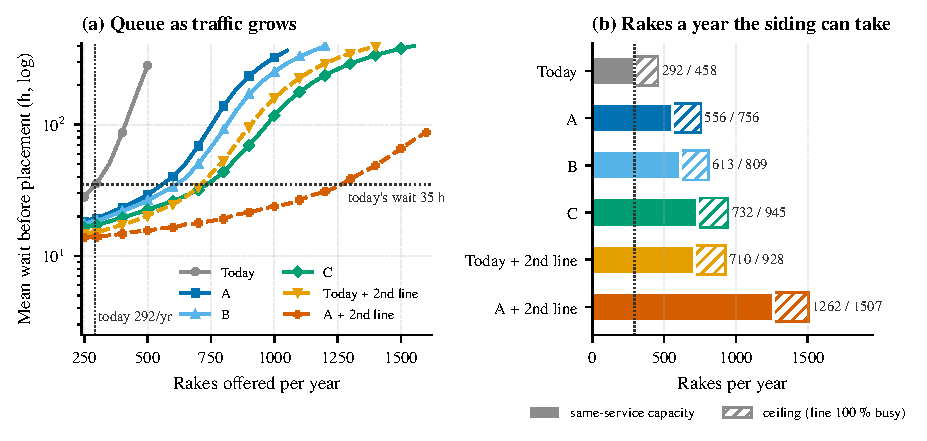
\includegraphics[width=0.94\textwidth]{figures/fig_capacity.pdf}
\caption[Queue and capacity of the coal siding as traffic grows]{Capacity of the coal siding (Layer 9, 30 replications $\times$ 200 rakes). (a) Mean wait before placement as the offered traffic grows; the dotted line is today's wait at 292 rakes a year. (b) Same-service capacity, Eq.~\eqref{eq:samesvc}, and capacity ceiling, Eq.~\eqref{eq:ceiling}.}
\label{fig:capacity}
\end{figure}

Today the siding works at 64\,\% line utilisation and rakes wait 35.0\,h before placement (the 200-rake runs of Layer 9 give 35.0\,h and a line hold of 19.1\,h, against 37.4\,h and 19.0\,h in the 50-rake runs of Table~\ref{tab:pack}; each comparison uses its own paired base). The queue grows steeply with traffic: at 400 rakes a year the wait passes 85\,h, and above the ceiling of 458 rakes a year the siding cannot clear what is offered (at 550 offered, only 448 a year are turned round). Table~\ref{tab:capacity} gives the capacity of each configuration.

\begin{table}[!htbp]
\centering
\caption[Capacity of the coal siding by configuration]{Capacity of the coal siding by configuration (Layer 9). Same-service capacity keeps the wait no longer than today's 35.0\,h.}
\label{tab:capacity}
\small
\begin{tabular}{@{}lrrrrr@{}}
\toprule
\textbf{Configuration} & \textbf{Line held} & \textbf{Ceiling} & \textbf{Same-} & \multicolumn{2}{c}{\textbf{Extra rakes vs today}} \\
\cmidrule(l){5-6}
 & \textbf{(h/rake)} & \textbf{(rakes/yr)} & \textbf{service} & \textbf{rakes/yr} & \textbf{\%} \\
\midrule
Today & 19.1 & 458 & 292 & -- & -- \\
A: paperwork 24/7, digital release & 11.6 & 756 & 556 & +264 & +90 \\
B: A + precise loading & 10.8 & 809 & 613 & +321 & +110 \\
C: B + faster loading & 9.3 & 945 & 732 & +440 & +151 \\
\midrule
Today + second line + second crew & 18.9 & 928 & 710 & +418 & +143 \\
A + second line + second crew & 11.6 & 1,507 & 1,262 & +970 & +332 \\
\bottomrule
\end{tabular}
\end{table}

Four findings follow.
\begin{enumerate}
    \item \textbf{Procedure nearly doubles capacity without construction.} Package A shortens the line hold from 19.1 to 11.6\,h, which raises the ceiling by 65\,\% (458 to 756 rakes a year) and lets the same line take 556 rakes a year at today's wait instead of 292 (+90\,\%). Package C, still without a new line, takes 732 (+151\,\%).
    \item \textbf{For capacity, a second line does matter.} Unlike detention, where a second line saved only 0.58\,h, capacity grows with the number of places to stand: a second line with a crew lifts same-service capacity to 710 rakes a year (+143\,\%), about the same as package C. The two kinds of lever are complements: procedure shortens each rake's stay, a line adds parallel service.
    \item \textbf{Combined, they multiply.} Package A with a second line and crew takes 1,262 rakes a year at today's wait, 4.3 times today's traffic, because each of two lines is also held for a shorter time.
    \item \textbf{More traffic does not raise detention or demurrage per rake.} Detention stays at about 17.0--17.5\,h (today) and 9.6\,h (A) at every traffic level, because it is set by paperwork, not by the queue. Under package A the siding could handle 550 rakes a year with a total demurrage bill of Rs 1.12 crore, against Rs 2.66 crore for 292 rakes today.
\end{enumerate}

\paragraph{What saturates first.} The line is the bottleneck in every configuration. At today's traffic the line is busy 64\,\% of the time, the loading crew 16\,\% and the shunting locomotive 7\,\%. Even at the same-service capacity of each configuration, the crew stays below 34\,\% and the locomotive below 29\,\% utilisation, so neither a second crew alone nor a second locomotive would add capacity until the line constraint is removed. The scaling question ``if traffic grows, what else must grow?'' therefore has a clear order: first shorten the line hold (procedure), then add a line with its crew; the locomotive and the crew follow much later.

\paragraph{Check against queueing theory.} The simulated queue was compared with the Pollaczek--Khinchine formula (Eq.~\eqref{eq:pk}) using the simulated line holds (Table~\ref{tab:pk}). With every office open, so that rakes reach the queue as a Poisson stream, the simulation agrees with the formula to within 0.91--1.03 times below 80\,\% line utilisation. With offices as modelled, the simulated queue is 1.04--1.96 times the formula below 80\,\% utilisation, highest for the packages with short line holds. The reason is mechanical: the forwarding note (M3) is cleared only in office hours, so rakes join the queue in bunches when the office opens, and bunched arrivals wait longer than Poisson ones. The check therefore confirms the queue mechanics and shows that office hours hurt twice: they lengthen each rake's stay and they bunch the arrivals.

\begin{table}[!htbp]
\centering
\caption[Simulated wait in the line queue against the Pollaczek--Khinchine formula]{Simulated wait in the line queue against the Pollaczek--Khinchine formula (Layer 9).}
\label{tab:pk}
\small
\begin{tabular}{@{}llrrrr@{}}
\toprule
\textbf{Configuration} & \textbf{Offices} & \textbf{Rakes/yr} & \textbf{Line use} & \textbf{Simulated (h)} & \textbf{Sim. / formula} \\
\midrule
Today & all open & 292 & 0.46 & 6.47 & 1.03 \\
Today & all open & 450 & 0.71 & 17.06 & 0.96 \\
A & all open & 292 & 0.39 & 3.90 & 1.01 \\
A & all open & 600 & 0.79 & 21.29 & 0.91 \\
\midrule
Today & as modelled & 292 & 0.64 & 21.96 & 1.15 \\
A & as modelled & 292 & 0.39 & 6.48 & 1.67 \\
C & as modelled & 292 & 0.31 & 4.31 & 1.96 \\
\bottomrule
\end{tabular}
\end{table}

The capacity figures rest on the same assumed paperwork times as the rest of the model, so they are read as directions and orders of magnitude: procedure roughly doubles the rakes a line can take, and procedure plus a second line roughly quadruples them.

\section{Wagon Damage and the Locomotive}
\label{sec:res_damage}
No published rate of wagon damage at loading sidings exists, so damage is an optional, assumed scenario (Section~\ref{sec:form}), following IR examination practice and audit findings \cite{irimee, cag}. Table~\ref{tab:dmg} compares the two rules for unfit wagons. Detaching the bad wagons adds a little detention, because the work falls inside the billed window. Returning the whole rake hardly changes the client's detention, because the rejected visit happens before the clock starts, but it costs the Railway about 2.3--2.6 times the wagon time of detaching. Detaching at the siding is the better rule for the system. The module measures time only; no repair price per wagon was available, so damage is not converted into rupees beyond its effect on demurrage.

\begin{table}[!htbp]
\centering
\caption[Extra hours per rake caused by defective wagons, coal siding today]{Extra hours per rake caused by defective wagons, coal siding today (Layer 8, assumed rates).}
\label{tab:dmg}
\small
\begin{tabular}{@{}lcccc@{}}
\toprule
 & \multicolumn{2}{c}{\textbf{Detach bad wagons}} & \multicolumn{2}{c}{\textbf{Return whole rake}} \\
\cmidrule(lr){2-3}\cmidrule(l){4-5}
\textbf{Defective wagons} & detention & arrival$\to$departure & detention & arrival$\to$departure \\
\midrule
0.5\,\% & +0.11 & +0.47 & +0.09 & +1.23 \\
1\,\% & +0.28 & +1.13 & +0.17 & +2.99 \\
2\,\% & +0.58 & +2.57 & +0.41 & +5.99 \\
\bottomrule
\end{tabular}
\end{table}

The shunting locomotive is modelled as a shared resource for placement, removal and detaching. A second locomotive saves no detention (Figure~\ref{fig:interv}) and the locomotive is busy at most 29\,\% of the time even at the highest same-service capacity (Section~\ref{sec:res_capacity}), so it is not a constraint in the modelled range. Locomotive breakdowns, late locomotives and the availability of train engines for the loaded haul are not modelled.

\section{Sufficiency of the Variable Set}
\label{sec:res_suff}
Layer 7 added each omitted factor of Table~\ref{tab:factors} at a realistic size, applied after the intervention so that no intervention can remove it, and re-ranked the six main interventions (Table~\ref{tab:suff}). The omitted factors change the \emph{level} of detention, from 15.5 to 23.1\,h with all of them together, but not the \emph{conclusions}: the ranking of the interventions is identical in all eight stress tests (Kendall $\tau = 1.00$), the best procedural lever saves 3.6--6.6 times as much as the best capital lever, and a second line without a crew never helps. The variable set is therefore sufficient for ranking interventions, the purpose of this study, though not for predicting absolute hours at a named siding.

\begin{table}[!htbp]
\centering
\caption[Omitted-factor stress test]{Omitted-factor stress test (Layer 7, 30 paired replications). Procedure / capital is the saving of the best procedural lever (digitalise all paperwork) divided by that of the best capital lever (faster loading).}
\label{tab:suff}
\small
\begin{tabular}{@{}lrcc@{}}
\toprule
\textbf{Omitted factor added} & \textbf{Base (h)} & \textbf{Kendall $\tau$} & \textbf{Proc./capital} \\
\midrule
None (model as built) & 15.53 & 1.00 & 4.4 \\
+1\,h physical delay inside free time & 17.00 & 1.00 & 4.8 \\
+3\,h physical delay inside free time & 19.99 & 1.00 & 5.3 \\
+1\,h unmodelled paperwork & 17.24 & 1.00 & 4.7 \\
+3\,h unmodelled paperwork & 20.68 & 1.00 & 5.4 \\
+50\,\% traffic & 15.87 & 1.00 & 4.7 \\
Loading disruptions (rate $-20$\,\%, sd $\times 2$) & 18.49 & 1.00 & 3.6 \\
Error rates $\times 2$ & 17.39 & 1.00 & 5.2 \\
All together & 23.07 & 1.00 & 6.6 \\
\bottomrule
\end{tabular}
\end{table}

\section{Summary: Time, Cost and Capacity}
\label{sec:res_summary}
Table~\ref{tab:summary} brings the three outcomes together for the coal siding. Package A, which needs no construction, nearly halves detention, cuts demurrage by more than three quarters, returns about 48 wagons to the fleet and nearly doubles the rakes the siding can take. Capital adds capacity but not speed; procedure adds both.

\begin{table}[!htbp]
\centering
\caption[Time, cost and capacity of the coal siding by package]{Time, cost and capacity of the coal siding by package (Layers 8 and 9).}
\label{tab:summary}
\small
\begin{tabular}{@{}lrrrr@{}}
\toprule
\textbf{Package} & \textbf{Detention (h)} & \textbf{Demurrage avoided} & \textbf{Wagons freed} & \textbf{Rakes/yr at today's wait} \\
 & & \textbf{(Rs crore/yr)} & & \\
\midrule
Today & 17.02 & -- & -- & 292 \\
A & 9.50 & 2.05 & 47.6 & 556 \\
B & 8.82 & 2.21 & 50.5 & 613 \\
C & 7.25 & 2.44 & 56.4 & 732 \\
\bottomrule
\end{tabular}
\end{table}

% ======================================================================
% CHAPTER 4  CONCLUSION
% ======================================================================
\chapter{Conclusion}
\label{ch:conclusion}

\section{Summary of Findings}
This report set out to find which operational, commercial and managerial constraints detain rolling stock at a freight terminal, and which interventions release it fastest, cheapest and with the most capacity gained. A layered, verified discrete-event simulation of a private coal siding was built, with IR charging rules cited from the source, every parameter tagged as cited or assumed, commodity attributes taken from 220,395 Eastern Railway freight records, and 107 automated checks. The main findings are:
\begin{enumerate}
    \item \textbf{Detention is mainly an administrative and managerial problem.} The calibrated siding detains a rake for 15.53\,h against 4.05\,h of physical work. About 78\,\% of rake waiting comes from office hours and rejected documents; better sequencing can recover at most 8\,\%, and 14\,\% is irreducible congestion.
    \item \textbf{Procedure beats capital for speed.} Digitalising the paperwork saves about 15.5 times more detention than a second line with a second crew (8.98\,h against 0.58\,h). A second line without a crew, a second shunting locomotive and pricing changes do not shorten detention.
    \item \textbf{One calendar decision dominates.} The hours a day the terminal's own paperwork runs move detention by 21.2\,h, more than all physical parameters together, and the first extra two hours give 43\,\% of the round-the-clock gain.
    \item \textbf{Money falls faster than time.} For a coal siding, round-the-clock terminal paperwork with digital release (package A, no construction) cuts detention from 17.0 to 9.5\,h (44\,\%) but demurrage by 78\,\%, Rs 2.05 crore a year, because the graded tariff charges the last hours most. Precise loading adds Rs 4.20 crore a year of avoided overload and unused-capacity loss, mostly as capacity.
    \item \textbf{Procedure also adds capacity; a second line adds more.} Package A lets the same line take 556 rakes a year at today's waiting time instead of 292 (+90\,\%); package C takes 732 (+151\,\%). A second line with a crew, which barely changes detention, lifts capacity to 710 rakes a year, and combined with package A to 1,262, 4.3 times today's traffic. The line is the bottleneck throughout; the crew and the locomotive stay below 34\,\% and 29\,\% utilisation.
    \item \textbf{The findings are general and robust.} The same general levers rank first for all ten commodities, while silo and precise loading are bulk-specific. The ranking of interventions is unchanged in eight omitted-factor stress tests (Kendall $\tau = 1.00$), and the simulated queue matches queueing theory when offices are open.
    \item \textbf{Damaged wagons should be detached, not the rake returned.} Returning the rake costs the Railway about 2.3--2.6 times the wagon time of detaching the bad wagons.
\end{enumerate}

\section{Recommendations}
\begin{itemize}
    \item \textbf{Terminal (siding owner):} run placement advice, weighment and release reporting round the clock, or at least extend the day from 16 to 18\,h as a first step; report release digitally; load to the permissible carrying capacity to avoid overload rework and penalties. This is the cheapest route to both lower demurrage and more rakes.
    \item \textbf{Capacity planning:} if traffic must grow beyond what package C can take (about 730 rakes a year at today's wait), add a second line \emph{with} its crew, after the procedural package; a second line without a crew, or a second locomotive, adds nothing first.
    \item \textbf{Railway:} support electronic placement advice and release reporting at the serving station, so the free-time clock reflects work rather than office hours; detach damaged wagons at the siding instead of returning the rake.
    \item \textbf{Client:} use electronic railway receipts and payment, which the data show are already the norm for coal, so the loaded rake is not held after removal.
\end{itemize}

\section{Limitations}
\begin{itemize}
    \item \textbf{Calibration, not validation.} Paperwork durations and rejection rates are assumed and tuned to TERI's 14--17\,h band, because no siding time logs were available. Rupee and capacity figures are therefore orders of magnitude; rankings and relations are the robust result.
    \item \textbf{Gross savings.} The cost of round-the-clock staffing, digital systems, weigh-controlled loading, silos or a second line is not yet subtracted, so no package has a payback figure yet.
    \item \textbf{Assumed scenarios.} Wagon damage rates and times are assumed, and damage is measured in time only, without a repair price.
    \item \textbf{Railway receipt basis.} The model's office-hours railway receipt (M7) conflicts with the data (electronic for 99.7\,\% of coal). This changes wagon time and attribution, not detention, demurrage or capacity; both bases are reported.
    \item \textbf{Scope.} One siding with one line is modelled; locomotive breakdowns, train-engine availability, line haul and network-level wagon allocation are outside the model.
\end{itemize}

\section{Future Work (MTP Part II)}
\begin{enumerate}
    \item \textbf{Validation on time logs:} fit the M4--M6 and loading times to siding placement--release logs (requested) and validate detention instead of calibrating it.
    \item \textbf{Net benefit and payback:} add implementation costs and rank packages by net benefit, payback period and cost per extra rake of capacity.
    \item \textbf{Capacity planning in depth:} extend Layer 9 to other commodities and to staged expansion (when to add the second line), and test traffic peaks and seasonality.
    \item \textbf{Railway receipt and paperwork:} recalibrate M7 to the electronic receipt and payment shares in the data, and add commodity-specific paperwork.
    \item \textbf{Wagon damage and the locomotive:} damage rates and repair costs by wagon type and material, and locomotive availability and breakdowns, with the supervisor's input on times and prices.
    \item \textbf{A tighter sequencing bound} through a time-indexed formulation \cite{sousa}.
\end{enumerate}


% ======================================================================
% REFERENCES
% ======================================================================
\renewcommand{\bibname}{References}
\begin{thebibliography}{99}
\addcontentsline{toc}{chapter}{References}
\small\setstretch{1.15}

\bibitem{azem}
Azem, S., Aggoune, R., \& Dauz\`ere-P\'er\`es, S. (2007). Disjunctive and time-indexed formulations for non-preemptive job shop scheduling with resource availability constraints. \textit{IEEE International Conference on Industrial Engineering and Engineering Management (IEEM)}.

\bibitem{campolongo}
Campolongo, F., Cariboni, J., \& Saltelli, A. (2007). An effective screening design for sensitivity analysis of large models. \textit{Environmental Modelling \& Software}, 22(10), 1509--1518.

\bibitem{cwc}
Central Warehousing Corporation, Railside Warehouse Complex handling tariffs (14 terminals); Bharat Coking Coal Ltd., Schedule of Rates 2025 (coal loading by payloader).

\bibitem{cag}
Comptroller and Auditor General of India (2014). \textit{Report No. 31 of 2014, Union Government (Railways)}, Chapter 10: Management of Goods Trains.

\bibitem{errr}
Eastern Railway (2022--2026). Inward freight register, railway-receipt base, monthly FOIS exports, January 2022 -- August 2026 (unpublished data).

\bibitem{graham}
Graham, R. L., Lawler, E. L., Lenstra, J. K., \& Rinnooy Kan, A. H. G. (1979). Optimization and approximation in deterministic sequencing and scheduling: a survey. \textit{Annals of Discrete Mathematics}, 5, 287--326.

\bibitem{gross}
Gross, D., Shortle, J. F., Thompson, J. M., \& Harris, C. M. (2008). \textit{Fundamentals of Queueing Theory} (4th ed.). Wiley.

\bibitem{guan}
Guan, C., \& Liu, R. (2009). Modeling gate congestion of marine container terminals, truck waiting cost, and optimization. \textit{Transportation Research Record}, 2100, 58--67.

\bibitem{irimee}
Indian Railways Institute of Mechanical and Electrical Engineering (IRIMEE). \textit{Freight train examination} (course material).

\bibitem{kendall}
Kendall, M. G. (1938). A new measure of rank correlation. \textit{Biometrika}, 30(1/2), 81--93.

\bibitem{law}
Law, A. M. (2015). \textit{Simulation Modeling and Analysis} (5th ed.). McGraw-Hill.

\bibitem{little}
Little, J. D. C. (1961). A proof for the queuing formula: $L = \lambda W$. \textit{Operations Research}, 9(3), 383--387.

\bibitem{ircomp}
Ministry of Railways (2024). \textit{Compendium: Demurrage, Stabling, Wharfage, Stacking, Waiver and Write-off}, as on 03.04.2024, under Rates Master Circular/Demurrage-Wharfage-Waiver/2016/0 dated 19.05.2016.

\bibitem{morris}
Morris, M. D. (1991). Factorial sampling plans for preliminary computational experiments. \textit{Technometrics}, 33(2), 161--174.

\bibitem{parmak}
Parmaksizoglou, I. A., Bombelli, A., \& Sharpanskykh, A. (2025). A multi-agent optimization approach for multimodal collaboration in marine terminals. \textit{Logistics}, 9(3), 110.

\bibitem{ortools}
Perron, L., \& Didier, F. CP-SAT solver, Google OR-Tools. \url{https://developers.google.com/optimization}

\bibitem{pib}
Press Information Bureau, Ministry of Coal (2024, 7 October). Union Minister of State for Coal and Mines Shri Satish Chandra Dubey lays the foundation stone of two projects of CCL.

\bibitem{raballand}
Raballand, G., Refas, S., Beuran, M., \& Isik, G. (2012). \textit{Why Does Cargo Spend Weeks in Sub-Saharan African Ports? Lessons from Six Countries}. World Bank, Directions in Development.

\bibitem{refas}
Refas, S., \& Cantens, T. (2011). Why does cargo spend weeks in Sub-Saharan African ports? The case of Douala, Cameroon. \textit{World Bank Policy Research Working Paper} 5565.

\bibitem{robinson}
Robinson, S. (2008). Conceptual modelling for simulation Part I: definition and requirements. \textit{Journal of the Operational Research Society}, 59(3), 278--290.

\bibitem{saltelli}
Saltelli, A., Ratto, M., Andres, T., Campolongo, F., Cariboni, J., Gatelli, D., Saisana, M., \& Tarantola, S. (2008). \textit{Global Sensitivity Analysis: The Primer}. Wiley.

\bibitem{sargent}
Sargent, R. G. (2013). Verification and validation of simulation models. \textit{Journal of Simulation}, 7(1), 12--24.

\bibitem{shapley}
Shapley, L. S. (1953). A value for n-person games. In H. W. Kuhn \& A. W. Tucker (Eds.), \textit{Contributions to the Theory of Games II} (pp. 307--317). Princeton University Press.

\bibitem{smith}
Smith, R. G. (1980). The Contract Net Protocol: High-level communication and control in a distributed problem solver. \textit{IEEE Transactions on Computers}, C-29(12), 1104--1113.

\bibitem{sousa}
Sousa, J. P., \& Wolsey, L. A. (1992). A time indexed formulation of non-preemptive single machine scheduling problems. \textit{Mathematical Programming}, 54, 353--367.

\bibitem{simpy}
Team SimPy. SimPy: discrete-event simulation for Python. \url{https://simpy.readthedocs.io}

\bibitem{teri}
TERI (2023). \textit{Strategies to Increase Railway's Share in Freight Transport in India, Vol. I: Terminal Operations and Development}. The Energy and Resources Institute, New Delhi.

\bibitem{wagonvalue}
ThePrint (2026, 29 October). Jupiter Wagons bags Rs 1,140 crore railway order for 2,583 wagons (PTI).

\bibitem{wco}
World Customs Organization (2018). \textit{Guide to Measure the Time Required for the Release of Goods (Time Release Study)}, Version 3. Brussels.

\end{thebibliography}


\end{document}
